% -*- Mode:TeX -*-

%% IMPORTANT: The official thesis specifications are available at:
%%            http://libraries.mit.edu/archives/thesis-specs/
%%
%%            Please verify your thesis' formatting and copyright
%%            assignment before submission.  If you notice any
%%            discrepancies between these templates and the 
%%            MIT Libraries' specs, please let us know
%%            by e-mailing thesis@mit.edu

%% The documentclass options along with the pagestyle can be used to
%% generate a technical report, a draft copy, or a regular thesis.  You
%% may need to re-specify the pagestyle after you \include cover.tex.
%% For more information, see the first few lines of mitthesis.cls.

%\documentclass[12pt,vi,twoside]{mitthesis}
%%
%%  If you want your thesis copyright to you instead of MIT, use the
%%  ``vi'' option, as above.
%%
%\documentclass[12pt,twoside,leftblank]{mitthesis}
%%
%% If you want blank pages before new chapters to be labelled ``This
%% Page Intentionally Left Blank'', use the ``leftblank'' option, as
%% above. 

\documentclass[12pt,twoside]{mitthesis}
\usepackage{lgrind}
%% These have been added at the request of the MIT Libraries, because
%% some PDF conversions mess up the ligatures.  -LB, 1/22/2014
\usepackage{cmap}
\usepackage[T1]{fontenc}

\usepackage{amssymb}
\usepackage{amsthm}
\theoremstyle{definition}

\usepackage{stmaryrd}
\usepackage{semantic}
\usepackage{stackrel}
\usepackage{minted}
\usepackage{caption}
\usepackage{subcaption}
\usepackage{color}

\pagestyle{plain}

%% This bit allows you to either specify only the files which you wish to
%% process, or `all' to process all files which you \include.
%% Krishna Sethuraman (1990).

%% \typein [\files]{Enter file names to process, (chap1,chap2 ...), or
%%   `all' to process all files:} \def\all{all} \ifx\files\all
%% \typeout{Including all files.} \else \typeout{Including only \files.}
%% \includeonly{\files} \fi

\begin{document}

% Some departments (e.g. 5) require an additional signature page.  See
% signature.tex for more information and uncomment the following line if
% applicable.
%% % -*- Mode:TeX -*-
%
% Some departments (e.g. Chemistry) require an additional cover page
% with signatures of the thesis committee.  Please check with your
% thesis advisor or other appropriate person to determine if such a 
% page is required for your thesis.  
%
% If you choose not to use the "titlepage" environment, a \newpage
% commands, and several \vspace{\fill} commands may be necessary to
% achieve the required spacing.  The \signature command is defined in
% the "mitthesis" class
%
% The following sample appears courtesy of Ben Kaduk <kaduk@mit.edu> and
% was used in his June 2012 doctoral thesis in Chemistry. 

\begin{titlepage}
\begin{large}
This doctoral thesis has been examined by a Committee of the Department
of Chemistry as follows:

\signature{Professor Jianshu Cao}{Chairman, Thesis Committee \\
   Professor of Chemistry}

\signature{Professor Troy Van Voorhis}{Thesis Supervisor \\
   Associate Professor of Chemistry}

\signature{Professor Robert W. Field}{Member, Thesis Committee \\
   Haslam and Dewey Professor of Chemistry}
\end{large}
\end{titlepage}


\pagestyle{plain}

\newcommand{\todo}[1]{\ensuremath{\textit{\textcolor{red}{TODO:}}\ \textrm{#1}}}

%% Definitions and theorems
\newtheorem{definition}{Definition}
\newtheorem{theorem}[definition]{Theorem}
\newtheorem{lemma}[definition]{Lemma}
\newtheorem{corollary}[definition]{Corollary}

\renewcommand\qedsymbol{$\blacksquare$}

%% Program keywords

\newcommand{\pgmcalls}{\ensuremath{\textbf{call}\ }}
\newcommand{\pgmif}{\ensuremath{\textbf{if}\ }}
\newcommand{\pgmthen}{\ensuremath{\textbf{then}\ }}
\newcommand{\pgmelse}{\ensuremath{\textbf{else}\ }}
\newcommand{\pgmlet}{\ensuremath{\textbf{let}\ }}
\newcommand{\pgmin}{\ensuremath{\textbf{in}\ }}
\newcommand{\pgmasserts}{\ensuremath{\textbf{assert}\ }}
\newcommand{\pgmrets}{\ensuremath{\textbf{ret}\ }}

\newcommand{\pgmmodule}[1]{\ensuremath{\textbf{Module}\ #1}}
\newcommand{\pgmregs}[1]{\ensuremath{\textbf{Regs}\ #1}}
\newcommand{\pgminsts}[1]{\ensuremath{\textbf{Instances}\ #1}}
\newcommand{\pgmrule}[1]{\ensuremath{\textbf{Rule}\ #1}}
\newcommand{\pgmmeth}[1]{\ensuremath{\textbf{Method}\ #1}}
\newcommand{\pgmameth}[1]{\ensuremath{\textbf{ActionMethod}\ #1}}

\newcommand{\pgmwrite}[2]{\ensuremath{#1 := #2\,;}\\}
\newcommand{\pgmcall}[3]{\ensuremath{#1 = \pgmcalls{} #2(#3)\,;}\\}
\newcommand{\pgmcalln}[2]{\ensuremath{\pgmcalls{} #1(#2)\,;}\\}
\newcommand{\pgmletin}[2]{\ensuremath{\pgmlet{} #1 = #2\ \pgmin{}}\\}
\newcommand{\pgmifelse}[4]{\ensuremath{\pgmif{} #1\ \pgmthen{} #2\ \pgmelse{} #3\,;}\\}
\newcommand{\pgmassert}[1]{\ensuremath{\pgmasserts{} #1\,;}\\}
\newcommand{\pgmret}[1]{\ensuremath{\pgmrets{} #1}\\}

%% BSV boxes by Murali

%% \newcommand{\bsvcodesize}{\footnotesize}
\newcommand{\bsvcodesize}{\small}

%BSV block
\newcommand{\bsvblock}[1]{
\ensuremath{
\begin{array}{@{\;\;\;\;\;\;}l}
#1
\end{array}}\\
}

%BSV normal rule
\newcommand{\bsv}[6]{
\begin{tabular}{@{}p{7cm}@{}}
\ensuremath{#1} {\it #2} #3:\\
\hline
\ensuremath{
\begin{array}{@{}l}
#4
\begin{array}{@{}l@{}l}
\when ( & 
#5) \pmb{\Rightarrow} \\
\end{array}\\
\bsvblock{#6}
\end{array}
}\\\\
\end{tabular}
}

%BSV rule without guard or let
\newcommand{\bsvnone}[4]{
\begin{tabular}{@{}p{7cm}@{}}
\ensuremath{#1} {\it #2} #3:\\
\hline
\ensuremath{
\begin{array}{@{}l@{}}
#4\\
\end{array}
}
\end{tabular}
}

%BSV rule without guard or let
\newcommand{\bsvnonesmall}[5]{
\begin{tabular}{@{}p{#5}@{}}
\ensuremath{#1} {\it #2} #3:\\
\hline
\ensuremath{
\begin{array}{@{}l@{}}
#4\\
\end{array}
}
\end{tabular}
}

%BSV module

\newcommand{\bsvmodinst}[3]{
\bsvcodesize
\centering
\begin{tabular}{|l|}
\hline\\
\pgmmodule{} #1:\\
\pgminsts \ensuremath{#2};\\[.5em]
\hline\\[-.5em]
#3\\
\hline
\end{tabular}
}

\newcommand{\bsvmod}[3]{
\bsvcodesize
\centering
\begin{tabular}{|l|}
\hline\\
\pgmmodule{} #1:\\
\pgmregs \ensuremath{#2};\\[.5em]
\hline\\[-.5em]
#3\\
\hline
\end{tabular}
}

\newcommand{\bsvmodnoreg}[2]{
\bsvcodesize
\centering
\begin{tabular}{|l|}
\hline\\
\pgmmodule{} #1:\\
\hline\\[-.5em]
#2\\
\hline
\end{tabular}
}

\newcommand{\bsvmodtbig}[3]{
\bsvcodesize
\centering
\begin{tabular}{|p{\textwidth}|}
\hline\\
\pgmmodule{}:\\
\pgmregs \ensuremath{#1};\\[.5em]
\hline\\[-.5em]
\begin{tabular}{cc}
\begin{minipage}{.5\textwidth}
#2
\end{minipage} &
\begin{minipage}{.5\textwidth}
#3
\end{minipage}
\end{tabular}\\
\hline
\end{tabular}
}

\newcommand{\bsvmodtsmall}[3]{
\bsvcodesize
\centering
\begin{tabular}{|p{\textwidth}|}
\hline\\[-.8em]
\pgmmodule{}:\\
\pgmregs \ensuremath{#1};\\[.2em]
\hline\\[-.5em]
\begin{tabular}{cc}
\begin{minipage}{.5\textwidth}
#2
\end{minipage} &
\begin{minipage}{.5\textwidth}
#3
\end{minipage}
\end{tabular}\\
\hline
\end{tabular}
}

%% Keywords
\newcommand{\ie}{\emph{i.e.,}}
\newcommand{\eg}{\emph{e.g.,}}

%% Proper names
\newcommand{\Bluespec}{Bluespec}
\newcommand{\Kami}{Kami}

%% For Latex convenience
\newcommand{\refchap}[1]{Chapter~\ref{#1}}
\newcommand{\refsect}[1]{Section~\ref{#1}}
\newcommand{\refdef}[1]{Definition~\ref{#1}}
\newcommand{\refthm}[1]{Theorem~\ref{#1}}
\newcommand{\reflem}[1]{Lemma~\ref{#1}}
\newcommand{\refcor}[1]{Corollary~\ref{#1}}
\newcommand{\reffig}[1]{Figure~\ref{#1}}

%% Sets
\newcommand{\setconst}{\ensuremath{\mathcal{C}}}
\newcommand{\setregs}{\ensuremath{\mathcal{R}}}
\newcommand{\setrules}{\ensuremath{\mathcal{L}}}
\newcommand{\setmeths}{\ensuremath{\mathcal{F}}}

%% Syntax
\renewcommand{\listof}[1]{\ensuremath{\overrightarrow{#1}}}
\newcommand{\fail}{\ensuremath{\textsf{fail}}}

\newcommand{\wordlet}{\ensuremath{\textsf{let}\ }}
\newcommand{\wordassert}{\ensuremath{\textsf{assert}\ }}
\newcommand{\wordret}{\ensuremath{\textsf{return}\ }}
\newcommand{\wordin}{\ensuremath{\textsf{in}\ }}
\newcommand{\wordif}{\ensuremath{\textsf{if}\ }}
\newcommand{\wordthen}{\ensuremath{\textsf{then}\ }}
\newcommand{\wordelse}{\ensuremath{\textsf{else}\ }}
\newcommand{\wordforeach}{\ensuremath{\textsf{foreach}\ }}

\newcommand{\tab}{\ensuremath{\quad}}

\newcommand{\seop}{\ensuremath{\textsf{op}}}
\newcommand{\eop}[1]{\ensuremath{\seop{}(\listof{#1})}}

\newcommand{\actwrite}[3]{\ensuremath{#1 := #2\,;\ #3}}
%% \newcommand{\actcall}[4]{\ensuremath{\wordlet{} #1 = #2(#3)\ \wordin{} #4}}
\newcommand{\actcall}[4]{\ensuremath{#2(#3)\,;\ \lambda #1.#4}}
%% \newcommand{\actlet}[3]{\ensuremath{\wordlet{} #2 = #1\ \wordin{} #3}}
\newcommand{\actlet}[3]{\ensuremath{\wordlet{} #1\ \wordin{} \lambda #2.#3}}
\newcommand{\actifelse}[5]{\ensuremath{\wordif{} #1\ \wordthen{} #2\ \wordelse{} #3\,;\ \lambda #4.#5}}
\newcommand{\actassert}[2]{\ensuremath{\wordassert{} #1\,;\ #2}}
\newcommand{\actret}[1]{\ensuremath{\wordret{} #1}}

\newcommand{\regpair}[2]{\ensuremath{(#1, #2)}}
\newcommand{\rulepair}[2]{\ensuremath{(#1, #2)}}
\newcommand{\methodpair}[2]{\ensuremath{(#1, #2)}}

\newcommand{\modbasic}[3]{\ensuremath{(\listof{#1}, \listof{#2}, \listof{#3})}}
\newcommand{\modcomp}[2]{\ensuremath{#1 \oplus #2}}
\newcommand{\modflatten}[1]{\ensuremath{\overline{\overline{#1}}}}

%% Semantics

\newcommand{\btrue}{\ensuremath{\textsf{true}}}
\newcommand{\bfalse}{\ensuremath{\textsf{false}}}
\newcommand{\band}{\ensuremath{\&\&}}

\renewcommand{\emptyset}{\ensuremath{\varnothing}}
\newcommand{\emptymap}{\ensuremath{[]}}
\newcommand{\finmapsymb}{\ensuremath{\stackrel{\textrm{\footnotesize{fin}}}{\longrightarrow}}}
\newcommand{\sttype}{\ensuremath{\setregs \finmapsymb \setconst}}
\newcommand{\lbtype}{\ensuremath{\setmeths \finmapsymb \setconst \times \setconst}}
\newcommand{\stupd}[3]{\ensuremath{#1 [ #2 \leftarrow #3 ]}}
\newcommand{\lblupd}[3]{\ensuremath{#1 [ #2 \leftarrow #3 ]}}
\newcommand{\setadd}[2]{\ensuremath{#1 \cup \{ #2 \}}}

\newcommand{\listnil}{\ensuremath{[]}}
\newcommand{\listcons}[2]{\ensuremath{#1::#2}}

\newcommand{\denot}[1]{\ensuremath{\llbracket #1 \rrbracket}}
\newcommand{\ssemexpr}[1]{\ensuremath{\denot{#1}_{\textsf{e}}}}
\newcommand{\semexpr}[2]{\ensuremath{\ssemexpr{#1}\ #2}}

\newcommand{\semact}[5]{\ensuremath{#1 |- (#2) \Downarrow \langle #3, #4, #5 \rangle}}
\newcommand{\semlbl}[3]{\ensuremath{\langle #1, #2, #3 \rangle}}
\newcommand{\semsstepr}[4]{\ensuremath{\langle #1, #2 \rangle \Downarrow \langle #3, #4 \rangle}}
\newcommand{\semsstep}[6]{\ensuremath{\langle #1, #2 \rangle \Downarrow \langle #3, \semlbl{#4}{#5}{#6} \rangle}}
\newcommand{\semsss}[4]{\ensuremath{\langle #1, #2 \rangle \Downarrow^{\ast} \langle #3, #4 \rangle}}
\newcommand{\semstep}[4]{\ensuremath{#2 \stackrel[#1]{#4}{\longrightarrow} #3}}

\newcommand{\Substep}{Substep}
\newcommand{\Substeps}{Substeps}
\newcommand{\Step}{Step}

\newcommand{\alpharule}[1]{\ensuremath{\textsf{Rule}\ #1}}
\newcommand{\alphameth}{\ensuremath{\textsf{Meth}}}

\newcommand{\namesof}[1]{\ensuremath{\textsf{namesOf}\ #1}}
\newcommand{\regsofm}[1]{\ensuremath{\textsf{regsOf}\ #1}}
\newcommand{\rulesofm}[1]{\ensuremath{\textsf{rulesOf}\ #1}}
\newcommand{\methsofm}[1]{\ensuremath{\textsf{methodsOf}\ #1}}
\newcommand{\callsofm}[1]{\ensuremath{\textsf{callsOf}\ #1}}
\newcommand{\callsofa}[1]{\ensuremath{\textsf{callsOfA}\ #1}}

\newcommand{\sdisj}[2]{\ensuremath{#1 \ast #2}}
\newcommand{\splus}[2]{\ensuremath{#1 \uplus #2}}
\newcommand{\sunion}[2]{\ensuremath{#1 \cup #2}}
\newcommand{\domof}[1]{\ensuremath{\textsf{domain}\ #1}}

\newcommand{\ldisj}[2]{\ensuremath{#1 \ast #2}}
\newcommand{\lplus}[2]{\ensuremath{#1 \uplus #2}}
\newcommand{\lunion}[2]{\ensuremath{#1 \cup #2}}

\newcommand{\annotof}[1]{\ensuremath{\textsf{annot}\ #1}}
\newcommand{\defsof}[1]{\ensuremath{\textsf{defs}\ #1}}
\newcommand{\callsof}[1]{\ensuremath{\textsf{calls}\ #1}}

\newcommand{\anndisj}[2]{\ensuremath{#1 \ast #2}}
\newcommand{\mdisj}[2]{\ensuremath{#1 \ast #2}}
\newcommand{\setdisj}[2]{\ensuremath{#1 \ast #2}}
\newcommand{\keysdisj}[2]{\ensuremath{\setdisj{\domof{#1}}{#2}}}

\newcommand{\annplus}[2]{\ensuremath{#1 \uplus #2}}
\newcommand{\mplus}[2]{\ensuremath{#1 \uplus #2}}

\newcommand{\wellhidden}[2]{\ensuremath{\textsf{wellHidden}\ #1\ #2}}
\newcommand{\hidesym}{\ensuremath{\textsf{hide}}}
\newcommand{\hide}[1]{\ensuremath{\hidesym{}\ #1}}
\newcommand{\hidemethsym}{\ensuremath{\textsf{hideMeth}}}
\newcommand{\hidemeth}[2]{\ensuremath{\hidemethsym{}\ #1\ #2}}
\newcommand{\hidemethssym}{\ensuremath{\textsf{hideMeths}}}
\newcommand{\hidemeths}[2]{\ensuremath{\hidemethssym{}\ #1\ #2}}

%% well-formedness

\newcommand{\wfdouble}[1]{\ensuremath{\textsf{WfDouble}\ #1}}
\newcommand{\wfdoubleap}[3]{\ensuremath{\textsf{WfDoubleA'}\ #1\ #2\ #3}}
\newcommand{\wfdoublea}[1]{\ensuremath{\textsf{WfDoubleA}\ #1}}

\newcommand{\wfcycle}[1]{\ensuremath{\textsf{WfCycle}\ #1}}

%% inlining

\newcommand{\concatsymb}{\ensuremath{::}}
\newcommand{\concataction}[2]{\ensuremath{#1 \concatsymb{} \lambda x.#2}}
\newcommand{\inlinedmsymb}{\ensuremath{\hookleftarrow}}
\newcommand{\inlinedm}[2]{\ensuremath{#1 \inlinedmsymb{} #2}}
\newcommand{\inlinedmssymb}{\ensuremath{\hookleftarrow^{\ast}}}
\newcommand{\inlinedms}[2]{\ensuremath{#1 \inlinedmssymb{} #2}}
\newcommand{\inlinedmmsymb}{\ensuremath{\hookleftarrow_{m}}}
\newcommand{\inlinedmm}[2]{\ensuremath{#1 \inlinedmmsymb{} #2}}
\newcommand{\inline}[1]{\ensuremath{| #1 |}}
\newcommand{\inlineF}[1]{\ensuremath{\| #1 \|}}

\newcommand{\isrec}[1]{\ensuremath{\textsf{isRecursive}\ #1}}

\newcommand{\mapfiltsymb}{\ensuremath{\smallsetminus}}
\newcommand{\mapfilt}[2]{\ensuremath{#1 \mapfiltsymb{} #2}}

\newcommand{\StepInl}{StepInl}
\newcommand{\semstepin}[4]{\ensuremath{#2 \stackrel[#1]{#4}{\hookrightarrow} #3}}

%% big-step semantics

\newcommand{\sembigact}[6]{\ensuremath{#1, #2 |- (#3) \leadsto \langle #4, #5, #6 \rangle}}
\newcommand{\sembigssr}[4]{\ensuremath{\langle #1, #2 \rangle \leadsto \langle #3, #4 \rangle}}
\newcommand{\sembigss}[6]{\ensuremath{\langle #1, #2 \rangle \leadsto \langle #3, \semlbl{#4}{#5}{#6} \rangle}}
\newcommand{\sembigstep}[4]{\ensuremath{#2 \stackrel[#1]{#4}{\leadsto} #3}}

\newcommand{\Bigsubstep}{BigSubstep}
\newcommand{\Bigstep}{BigStep}



%% % -*-latex-*-
% 
% For questions, comments, concerns or complaints:
% thesis@mit.edu
% 
%
% $Log: cover.tex,v $
% Revision 1.8  2008/05/13 15:02:15  jdreed
% Degree month is June, not May.  Added note about prevdegrees.
% Arthur Smith's title updated
%
% Revision 1.7  2001/02/08 18:53:16  boojum
% changed some \newpages to \cleardoublepages
%
% Revision 1.6  1999/10/21 14:49:31  boojum
% changed comment referring to documentstyle
%
% Revision 1.5  1999/10/21 14:39:04  boojum
% *** empty log message ***
%
% Revision 1.4  1997/04/18  17:54:10  othomas
% added page numbers on abstract and cover, and made 1 abstract
% page the default rather than 2.  (anne hunter tells me this
% is the new institute standard.)
%
% Revision 1.4  1997/04/18  17:54:10  othomas
% added page numbers on abstract and cover, and made 1 abstract
% page the default rather than 2.  (anne hunter tells me this
% is the new institute standard.)
%
% Revision 1.3  93/05/17  17:06:29  starflt
% Added acknowledgements section (suggested by tompalka)
% 
% Revision 1.2  92/04/22  13:13:13  epeisach
% Fixes for 1991 course 6 requirements
% Phrase "and to grant others the right to do so" has been added to 
% permission clause
% Second copy of abstract is not counted as separate pages so numbering works
% out
% 
% Revision 1.1  92/04/22  13:08:20  epeisach

% NOTE:
% These templates make an effort to conform to the MIT Thesis specifications,
% however the specifications can change.  We recommend that you verify the
% layout of your title page with your thesis advisor and/or the MIT 
% Libraries before printing your final copy.
\title{An Inlining Approach to Formal Hardware Semantics}

\author{Joonwon Choi}
% If you wish to list your previous degrees on the cover page, use the 
% previous degrees command:
%       \prevdegrees{A.A., Harvard University (1985)}
% You can use the \\ command to list multiple previous degrees
%       \prevdegrees{B.S., University of California (1978) \\
%                    S.M., Massachusetts Institute of Technology (1981)}
\prevdegrees{B.S., Seoul National University (2013)}
\department{Department of Electrical Engineering and Computer Science}

% If the thesis is for two degrees simultaneously, list them both
% separated by \and like this:
% \degree{Doctor of Philosophy \and Master of Science}
\degree{Master of Science in Electrical Engineering and Computer Science}

% As of the 2007-08 academic year, valid degree months are September, 
% February, or June.  The default is June.
\degreemonth{June}
\degreeyear{2016}
\thesisdate{May 19, 2016}

%% By default, the thesis will be copyrighted to MIT.  If you need to copyright
%% the thesis to yourself, just specify the `vi' documentclass option.  If for
%% some reason you want to exactly specify the copyright notice text, you can
%% use the \copyrightnoticetext command.  
%\copyrightnoticetext{\copyright IBM, 1990.  Do not open till Xmas.}

% If there is more than one supervisor, use the \supervisor command
% once for each.
\supervisor{Arvind}
           {Professor of Electrical Engineering and Computer Science}

% This is the department committee chairman, not the thesis committee
% chairman.  You should replace this with your Department's Committee
% Chairman.

\chairman{Professor Leslie A. Kolodziejski}
         {Chair, Department Committee on Graduate Students}

% Make the titlepage based on the above information.  If you need
% something special and can't use the standard form, you can specify
% the exact text of the titlepage yourself.  Put it in a titlepage
% environment and leave blank lines where you want vertical space.
% The spaces will be adjusted to fill the entire page.  The dotted
% lines for the signatures are made with the \signature command.
\maketitle

% The abstractpage environment sets up everything on the page except
% the text itself.  The title and other header material are put at the
% top of the page, and the supervisors are listed at the bottom.  A
% new page is begun both before and after.  Of course, an abstract may
% be more than one page itself.  If you need more control over the
% format of the page, you can use the abstract environment, which puts
% the word "Abstract" at the beginning and single spaces its text.

%% You can either \input (*not* \include) your abstract file, or you can put
%% the text of the abstract directly between the \begin{abstractpage} and
%% \end{abstractpage} commands.

% First copy: start a new page, and save the page number.
\cleardoublepage
% Uncomment the next line if you do NOT want a page number on your
% abstract and acknowledgments pages.
% \pagestyle{empty}
\setcounter{savepage}{\thepage}
\begin{abstractpage}
% $Log: abstract.tex,v $
% Revision 1.1  93/05/14  14:56:25  starflt
% Initial revision
% 
% Revision 1.1  90/05/04  10:41:01  lwvanels
% Initial revision
% 
%
%% The text of your abstract and nothing else (other than comments) goes here.
%% It will be single-spaced and the rest of the text that is supposed to go on
%% the abstract page will be generated by the abstractpage environment.  This
%% file should be \input (not \include 'd) from cover.tex.

Hardware components are extremely complex due to concurrency.
Modularity has been considered as an effective way to design and
understand such complex hardware components. Among various Hardware
Description Languages (HDLs), \Bluespec{} allows designers to develop
hardware not only based on modularity, but also based on the notion of
Guarded Atomic Actions (GAAs). Following the concepts of modularity
and GAA, we have been defining a framework called \Kami{}, which is
for specifying, verifying, and synthesizing \Bluespec{}-style hardware
components. However, modular semantics has an inherent weakness in
that it is hard to infer internal changes. In this thesis, I present a
new semantic approach based on inlining. Inlining semantics is defined
for open hardware systems and resolves the weakness by construction.
An implication from modular semantics to inlining semantics is also
formally proven, thus the inlining semantics can be used to
efficiently prove hardware properties.


\end{abstractpage}

% Additional copy: start a new page, and reset the page number.  This way,
% the second copy of the abstract is not counted as separate pages.
% Uncomment the next 6 lines if you need two copies of the abstract
% page.
% \setcounter{page}{\thesavepage}
% \begin{abstractpage}
% % $Log: abstract.tex,v $
% Revision 1.1  93/05/14  14:56:25  starflt
% Initial revision
% 
% Revision 1.1  90/05/04  10:41:01  lwvanels
% Initial revision
% 
%
%% The text of your abstract and nothing else (other than comments) goes here.
%% It will be single-spaced and the rest of the text that is supposed to go on
%% the abstract page will be generated by the abstractpage environment.  This
%% file should be \input (not \include 'd) from cover.tex.

Hardware components are extremely complex due to concurrency.
Modularity has been considered as an effective way to design and
understand such complex hardware components. Among various Hardware
Description Languages (HDLs), \Bluespec{} allows designers to develop
hardware not only based on modularity, but also based on the notion of
Guarded Atomic Actions (GAAs). Following the concepts of modularity
and GAA, we have been defining a framework called \Kami{}, which is
for specifying, verifying, and synthesizing \Bluespec{}-style hardware
components. However, modular semantics has an inherent weakness in
that it is hard to infer internal changes. In this thesis, I present a
new semantic approach based on inlining. Inlining semantics is defined
for open hardware systems and resolves the weakness by construction.
An implication from modular semantics to inlining semantics is also
formally proven, thus the inlining semantics can be used to
efficiently prove hardware properties.


% \end{abstractpage}

\cleardoublepage

\section*{Acknowledgments}

I would like to thank a number of people who have been contributing to
this work or who gave me thoughtful advices. Without help from these
people, I would not have been able to develop the work and to write
the thesis.

First, I would like to thank my advisors, Professor Arvind and Adam
Chlipala for giving me a significant amount of intuitions and
motivations about the work. Before joining the master degree program,
I had almost no experience on hardware verification. Thanks for
advices from Arvind and Adam, I learned a lot of knowledge and skills
fast and efficiently.

I would also like to thank the CSG and PLV group people for invaluable
advices. I specially give my gratitude to Muralidaran Vijayaraghavan
for discussing and developing the \Kami{} project together.

Last but not least, I would like to thank Kwanjeong Educational
Foundation, who supported me financially for the master degree.

%%%%%%%%%%%%%%%%%%%%%%%%%%%%%%%%%%%%%%%%%%%%%%%%%%%%%%%%%%%%%%%%%%%%%%
% -*-latex-*-

%%   % -*- Mode:TeX -*-
%% This file simply contains the commands that actually generate the table of
%% contents and lists of figures and tables.  You can omit any or all of
%% these files by simply taking out the appropriate command.  For more
%% information on these files, see appendix C.3.3 of the LaTeX manual. 
\tableofcontents
\newpage
\listoffigures
%% \newpage
%% \listoftables



%% \chapter{Introduction}

Hardware components are extremely complex. The main reasons for the
complexity is concurrency and the sheer size of components. For
example, realistic processors make use of instruction pipelining to
execute multiple instructions concurrently. Complexity comes with such
executions, since one must ensure that the concurrent executions
should behave as if they are executed in order. Size of components
also grows by complexity. More realistic processors require additional
hardware components such as a reorder buffer. The logic gets
complicated again with these components.

Modularity has been considered as an effective way to design and
understand such complex hardware components. A complex hardware
component can can be constructed by composing several simple
modules. The notion of modules is so ingrained in that all commercial
Hardware Description Languages (HDLs) like Verilog, VHDL, Bluespec,
and Chisel~\cite{verilog, vhdl, bsdef, chisel} support the notion of
modules.

Among various HDLs, \Bluespec{}~\cite{bsdef, bsref} allows designers
to develop hardware not only based on modularity, but also based on
the notion of Guarded Atomic Actions (GAAs)~\cite{daniel-gaa}. Even
though most HDLs allow to design hardware in a modular manner, modules
cannot be independently designed if they are entangled with
clock-timing issues. For instance, when two modules, a producer of a
value and a consumer of that value, are connected with wires and the
producer is optimized to use fewer clock cycles to produce the value,
then the consumer should also be modified to consume the values
faster; failure to do so will result in an incorrect overall design.

Following the concepts of modularity and GAA, we have been defining a
framework called \Kami{}~\cite{kami-web, murali-thesis}, which is for
specifying, verifying, and synthesizing \Bluespec{}-style hardware
components. \Kami{} presents a domain specific language similar to
Bluespec. In addition, we define the formal semantics of the \Kami{}
language to enable proving properties of hardware. The framework has
been built on the Coq proof assistant; hence verification can be
performed by mechanized proofs with a high degree of automation.

The notion of modularity used in designing hardware can be extended to
verification. For modular verification, we want to be able to verify
the individual modules of a large system and compose their proofs to
verify the full system. In many cases, we reuse such simple components
in different larger designs. From the perspective of proof, reusing a
hardware component implies that we can also reuse its related
proofs. Thanks to the modular semantics in \Kami{}, it is indeed
possible to use the proof of a component whenever it is used in a
larger design.

Modules communicate with other modules by calling each other's
methods. In our modular semantics, we model these communications using
\emph{labels}. The semantics of these communicating modules is similar
to those of Labeled Transition Systems (LTS)~\cite{lts}. Each module
changes its internal state and potentially calls methods of other
modules during its state transition. These method calls become labels
in our semantics.  The modular semantics, therefore, also defines
behaviors of \emph{open systems}. Open systems have external
interactions, whose specifics cannot be figured out unless it is
connected with other modules which can respond to them.

However, modular semantics has an inherent weakness in that it is hard
to infer internal changes. Even if modular semantics allow us to
consider individual modules, we eventually should be able to
understand a part of design which is still composed of several
modules, when the part cannot be decomposed anymore. Modular semantics
defines behaviors of such modules by giving the behaviors of each
small module. In this case, we should consider \emph{all possible
  combinations} of the small module behaviors. However, we certainly
do not want to consider all such cases, since we know only a few cases
are feasible by the design itself.

Hence, in this thesis, I present a new semantic approach, which is
based on inlining. Inlining semantics is defined for open hardware
systems and resolve the weakness by construction. The semantics uses a
static inlining operation to substitute internal calls to their method
bodies. This operator erases all internal calls in a module, so that
we do not need to care about internal communications.

An implication from the modular semantics to the inlining semantics is
also formally proven, thus it can be used in order to efficiently
prove properties of hardware. Since the two semantics does not have
equal capabilities, we give the implication proof saying that the
modular semantics imply the inlining semantics.

To sum up, the main contributions of this thesis are:
\begin{itemize}
\item To define a new semantic approach based on inlining, for open
  hardware systems.
\item To prove the implication from the modular semantics to the
  inlining semantics.
\end{itemize}

\paragraph{Overview}

The thesis is organized as follows: \refchap{chap:backgrounds}
introduces a number of prerequisites to understand the hardware design
concept of \Bluespec{}. Related works are also provided to compare
previous approaches to define hardware semantics.
\refchap{chap:semantics} presents the two semantics used in the
\Kami{} framework: modular and inlining
semantics. \refchap{chap:implication} compares capability of each
semantics and presents the implication proof between them. Lastly, we
draw conclusions and give future works in \refchap{chap:conclusions}.


%% \chapter{Backgrounds}
\label{chap:backgrounds}

\section{Hardware Design Paradigms}
\label{sec:design-paradigm}

Traditional Register-Transfer Level (RTL) designs require hardware
designers to consider scheduling for all resources. During hardware
design, one has to ensure that any resource elements are correctly
employed, e.g., one should not write a register more than once in the
same cycle, which would cause incorrect assignment. If a particular
input port of a hardware component is used more than once, we do not
have any guarantees for the output value, also causing incorrect use
of values. A well-known RTL design framework, Verilog, lets users take
responsibility for this, thus one should carefully investigate if
there is an assignment which makes an incorrect state transition.
\begin{figure}[h]
  \centering
  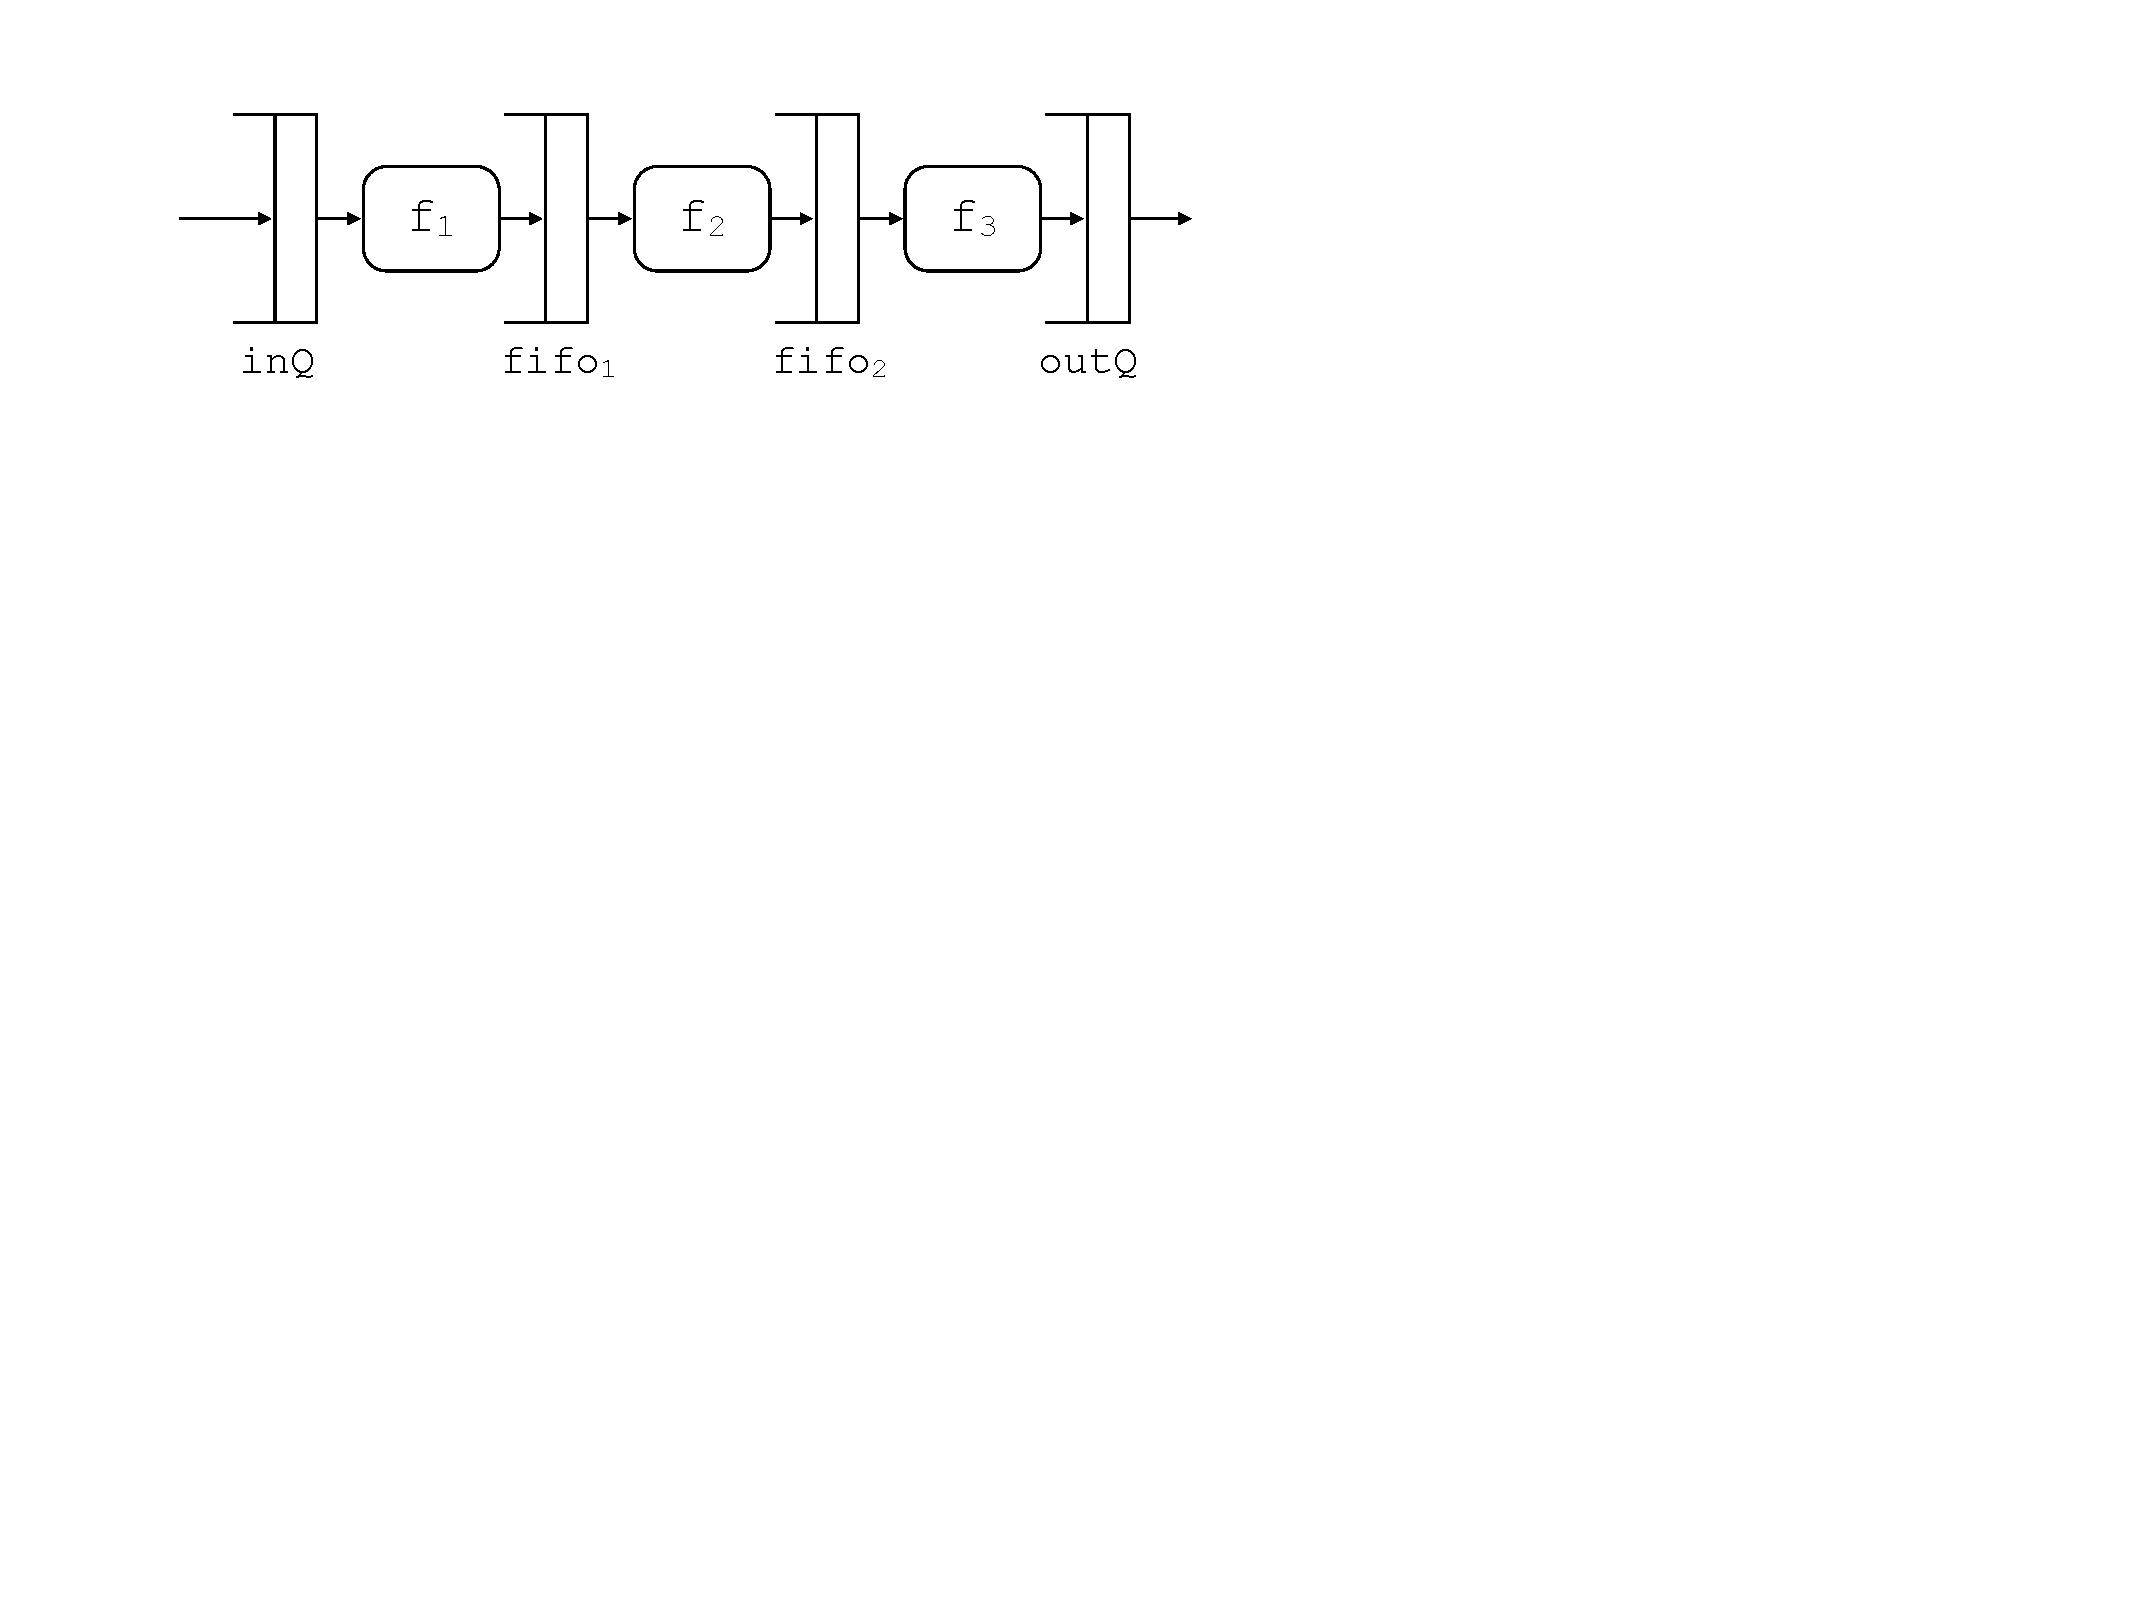
\includegraphics[width=0.5\textwidth]{figures/pipeline.pdf}
  \caption{A pipelined system}
  \label{fig-pipelined-system}
\end{figure}

A disadvantage of this approach is that having no separation between
functional parts and scheduling logic makes maintenance harder. Let us
revisit the pipelined system where three systems $f_1$, $f_2$, and
$f_3$ are connected by fifos, as shown in
\reffig{fig-pipelined-system}. For simplicity, suppose that only one
element can reside in a fifo. Since there is only one element in a
fifo, push and pop cannot be requested in the same cycle -- it will
cause double-write. Now the problem occurs because we have no
information whether push and pop will be requested simultaneously or
not. Thus in this case, we cannot avoid an implementation tightly
coupled with scheduling logic; for each case of push and pop, there is
no way for user except to define different implementations.

For this reason, in some frameworks like Verilog, designers tend to
specify the data path first, and then to define the controlling logic
which is entangled with the data path design. The problem with this
conventional design approach is that it is not flexible in perspective
of verification. If a designer specifies the controlling logic clearly
for a specific hardware system, it would be easy to verify
it. However, since that specification is only for one hardware system,
the verification approach used for the system may not be reusable for
other systems.

Guarded Atomic Action (GAA) is a design paradigm for correct and
effective scheduling that makes up for shortcomings of the RTL
designs. It is different from the traditional RTL designs mentioned
above. The main idea is that any hardware system has a (structural)
state component that can be captured by a set of variables that
represent registers or storage. State transition is done by a set of
rules, where a rule is a series of actions with \emph{guards} on this
state. A guard of a rule is a predicate that should be satisfied to
execute the rule. Each action (including one for rules) should be
atomic -- an execution of an action should be guaranteed to make a
state transition purely caused by the action.

\section{Semantics of the Bluespec Language}
\label{sec:bluespec-semantics}

\paragraph{Module structure}

Modularity forms the base semantics of the \Bluespec{} language. It is
simply to follow a natural hardware design concept. Hardware designers
usually design complex hardware components in a modular manner; small
module components are firstly designed, and they are composed to build
a large and complex one.

Bluespec also supports module definition. Each module has a set of
registers, called an \emph{internal state} of the module. The internal
state can be modified only by the module itself. In order to induce a
state change from the outside of the module, it should be requested by
method calls. The module also has a set of \emph{rules}. Each rule is
composed of GAAs. Rules are executed by a global rule scheduler. The
scheduler selects the maximal number of rules where the guards do not
conflict each others. Once the scheduler confirms the validity of the
guards, then they can be executed concurrently. Lastly, the module has
a set of \emph{methods}. Bluespec separates the notion of
\emph{Method} and \emph{ActionMethod}. Method is like a macro, which
evalutes an expression. From the perspective of hardware, Method can
be synthesized to a combinational circuit.  Whereas, ActionMethod is
composed of GAAs, and it only can be called by external modules. Thus,
it acts like an interface of the module, since ActionMethod is the
only way to manipulate internal states.

\begin{figure}[t]
  \centering{
    \begin{subfigure}[b]{0.5\textwidth}
      \bsvmodinst{PipelinedSystem}{inQ, fifo1, fifo2, outQ}{
        \bsvnone{\pgmrule}{stage0}{}{
          \pgmif{} \textrm{inQ.empty \&\& fifo1.notFull} \\
          \pgmthen{} \textrm{fifo1.enq(f0(inQ.first)); inQ.deq;}
        }\\
        \bsvnone{\pgmrule}{stage1}{}{
          \pgmif{} \textrm{fifo1.notEmpty \&\& fifo2.notFull} \\
          \pgmthen{} \textrm{fifo2.enq(f1(fifo1.first)); fifo1.deq;}
        }\\
        \bsvnone{\pgmrule}{stage2}{}{
          \pgmif{} \textrm{fifo2.notEmpty \&\& outQ.notFull} \\
          \pgmthen{} \textrm{outQ.enq(f2(fifo2.first)); fifo2.deq;}
        }\\
        \bsvnone{\pgmameth}{req}{(x)}{
          \textrm{inQ.enq(x);}
        }\\
        \bsvnone{\pgmameth}{res}{}{
          \pgmletin{x}{outQ.first}
          \textrm{outQ.deq;} \\
          \pgmret{x}
        }
      }
    \end{subfigure}
  }
  \caption{The pipelined system implemented with Bluespec}
  \label{ex-pipelined-system-bluespec}
\end{figure}

\reffig{ex-pipelined-system-bluespec} describes the psuedo-code
Bluespec module definition of the pipelined system shown in
\reffig{fig-pipelined-system}. The big module PipelinedSystem has four
module instances, named inQ, fifo1, fifo2, and outQ. It has three
rules (stage0, stage1, and stage2); each rule pulls an element from a
certain fifo, applies an operation, and push the resulting value into
the next fifo. The module has two interface methods: ``req'' is called
when there is a request with argument ``x'', and ``res'' is called to
get the result value.

\paragraph{Well-formedness of a module}

Syntactic correctness of a module does not imply the correct
execution. In other words, the module should satisfy an additional
number of conditions in order for valid execution. Firstly, a rule or
a method should not perform a write operation to the same register
twice (double-write). It also should not call the same method twice
(double-call). This is simply because actions in a rule (a method) are
executed simultaneously. A second condition is that method calls
cannot form a cycle among modules, since the cycle has no valid
behaviors in terms of hardware design. The last condition is that
register reads and writes should be defined within the module in which
the register is defined.

These conditions are sometimes called a well-formedness of a
module. It is usually defined independently with the semantics
definition, since it can be captured statically by traversing the
module definition. We formally define the well-formedness on
\refsect{sec-wf}, and use it on the correctness proof of an inlining
operation. See the section for more details.

\paragraph{Concurrent rule executions}

A guard of a rule includes which registers are written and which
methods are called. Double-writes and double-calls are caught by
forcing the well-formedness condition within a rule or a
method. \todo{explain}.

For instance, all the rules of PipelinedSystem can be executed
concurrently. In other words, the rule scheduler can verify that the
guards of the three rules in PipelinedSystem do not conflict. As
mentioned earlier, this is because the rules do not write the same
register and do not call the same method. \todo{more}.

\paragraph{One-rule-at-a-time semantics}

\section{Related Works: Previous Semantics Design}
\label{sec:related-works}

%% Nirav big-step semantics

%% Murali modular semantics

%% Any papers about inlining? Dan's thesis!! inlining used for merging
%% modules.


%% \chapter{An Inlining Approach to Hardware Semantics}
\label{chap:semantics}

In this chapter, we present a formal definition of inlining.  First,
we define the inlining operation on the \Kami{} language and the
modular semantics~\cite{murali-thesis}. We then present a new semantic
approach, which is based on the inlining operation.

\paragraph{Notations}

Before defining syntax and semantics, we introduce a number of
notations to represent general data structures.
\begin{itemize}
\item Lists: we use a symbol $\vec{t}\;$ to represent a type of list
  whose elements are represented as a value $t$. \listnil{} represents
  the nil list, and $(\listcons{hd}{tl})$ represents the list with a
  head $hd$ and a tail $tl$.
\item Sets: \emptyset{} represents an empty set, $(s \cup t)$
  represents the union of sets $s$ and $t$. $(a \in S)$ denotes an
  element $a$ in set $S$.
\item Finite maps: we use a symbol $(K \finmapsymb V)$ to represent a
  finite map with a set of keys $K$ and a set of values
  $V$. \emptymap{} represents an empty map, and $\stupd{m}{k}{v}$
  represents a map update with a new key $k$ and a value
  $v$. Singletons are represented by
  $\stupd{}{k}{v}$. $(\mapfilt{m}{ks})$ represents a map where all
  elements whose keys are in the list $ks$ are removed from $m$. We
  use the notation $\in$ also for finite maps to represent that a map
  has a certain key; $(k \in m)$ means that a map $m$ has a value for
  a key $k$.
\end{itemize}

\section{Syntax}

\paragraph{Expressions}
We begin by defining syntax for expressions. Expressions consist of
constant, register read, variable, and an inductive operation among
expressions.

\begin{definition}
  \label{def-expression}
  An expression $e$ is defined inductively as follows:
  \begin{center}
    \begin{math}
      \begin{array}{rcll}
        \textrm{Expression}\quad e & ::= & c & \textrm{(constant)} \\
        & | & r & \textrm{(register read)} \\
        & | & x & \textrm{(variable)} \\
        & | & \eop{e} & \textrm{(operation)} \\
      \end{array}
    \end{math}
  \end{center}
\end{definition}

Constants denote all concrete values used in hardware design. A number
of constants with different bit-widths may exist in real hardware
design, but they are abstracted into a single type for
convenience. Let \setconst{} be the set of such constants. $c \in
\setconst{}$ will be used as a typical character representing a
constant throughout the chapter.

$r \in \setregs{}$ in expressions represents the value of a register
$r$, where \setregs{} is the set of register names. $x$ denotes a
variable bound by a continuation. We define syntax as a
continuation-passing style (CPS), hence variables are used to get the
value of a continuation argument. Lastly, \eop{e} abstracts all
operations among expressions.

\paragraph{Actions}
As explained in \refsect{sec:design-paradigm}, an action is a unit for
describing hardware behaviors, which should ensure atomicity. Actions
consist of register write, method call, let bind, conditional branch,
assert, and return.

\begin{definition}
  \label{def-action}
  An action $a$ is defined inductively as follows:
  \begin{center}
    \begin{math}
      \begin{array}{rcll}
        \textrm{Action}\quad a & ::= & \actwrite{r}{e}{a} & \textrm{(register write)} \\
        & | & \actcall{x}{f}{e}{a} & \textrm{(method call)} \\
        & | & \actlet{e}{x}{a} & \textrm{(let bind)} \\
        & | & \actifelse{e}{a}{a}{x}{a} & \textrm{(conditional branch)} \\
        & | & \actassert{e}{a} & \textrm{(assert)} \\
        & | & \actret{e} & \textrm{(return)} \\
      \end{array}
    \end{math}
  \end{center}
\end{definition}

A register write action takes a register name $r$ and an expression
$e$ to assign the evaluated value of $e$ to $r$. A method call action
takes a method name $f \in \setmeths{}$ to call, and an expression $e$
as an argument. A return value for the call is bound to a variable $x$
in a lambda continuation. \setmeths{} denotes the set of method
names. A let bind action gives a name to an expression $e$. The name
is bound to a variable $x$ in a lambda continuation. A conditional
branch action similarly has a lambda binder $x$ to capture the return
value from true and false branches. An assert action takes an
expression $e$ to be checked to progress the continuation. Lastly, a
return action takes $e$ as a return value.

Even if actions are defined in a sequential manner, they are in fact
executed concurrently. Semantically, all inference rules for actions
will use the current state to obtain values from registers, which implies
that no actions use any updated values during the execution (see
\refdef{def-semaction} for details).

Due to the concurrent execution concept, when we \emph{concatenate}
two arbitrary action sequences, we can easily imagine the behavior of
the concatenated actions simply by merging two corresponding
behaviors. The action concatenation is used for various purposes such
as inlining a method body. \refdef{def-concataction} defines a
syntactic action concatenation operator. A semantic property will be
proven in \reflem{lem-concatsymb}.

\begin{definition}
  \label{def-concataction}
  $(\concatsymb) : \textrm{Action} \to \textrm{Action} \to
  \textrm{Action}$ is an infix operator, defined inductively with
  respect to the left-hand side action:
  \begin{center}
    \begin{math}
      \begin{array}{rcl}
        \concataction{(\actwrite{r}{e}{a})}{a_c} & \triangleq & \actwrite{r}{e}{(\concataction{a}{a_c})} \\
        \concataction{(\actcall{x}{f}{e}{a})}{a_c} & \triangleq & \actcall{x}{f}{e}{(\concataction{a}{a_c})} \\
        \concataction{(\actlet{e}{x}{a})}{a_c} & \triangleq & \actlet{e}{x}{(\concataction{a}{a_c})} \\
        \concataction{(\actifelse{e}{a_t}{a_f}{x}{a})}{a_c} & \triangleq &
        \actifelse{e}{a_t}{a_f}{x}{(\concataction{a}{a_c})} \\
        \concataction{(\actassert{e}{a})}{a_c} & \triangleq & \actassert{e}{(\concataction{a}{a_c})} \\
        \concataction{(\actret{e})}{a_c} & \triangleq & \actlet{e}{x}{a_c} \\
      \end{array}
    \end{math}
  \end{center}
\end{definition}

The only nontrivial definition comes from the return statement
$(\actret{e})$. Concatenating two actions involves to pass the return
value of the left action to the right action as an argument. However,
a dynamic evaluation of an expression cannot be involved with the
static concatenation operation. The problem can be solved by using
$\textsf{let}$ syntax structure, saying that we declare a name in
which $e$ is bound, and the value is used in the body ($\lambda
x.a_c$). Considering the semantic rule for $\textsf{let}$, it is
natural to define concatenation in such a way.

\paragraph{Modules}
A module is a unit of hardware systems which has its own state (a set
of registers), rules to induce internal state changes, and methods to
communicate with other modules.

\begin{definition}
  \label{def-module}
  A module $m$ is inductively defined as follows:
  \begin{center}
    \begin{math}
      \begin{array}{rcll}
        \textrm{Module}\quad m & ::=
        & \modbasic{\regpair{r}{c}}{\rulepair{s}{a}}{\methodpair{f}{\lambda x.a}}
        & \textrm{(basic module)} \\
        & | & \modcomp{m}{m} & \textrm{(composed module)}
      \end{array}
    \end{math}
  \end{center}
\end{definition}

A module is either a \emph{basic module} or a \emph{composed module}.
In a basic module, $\listof{\regpair{r}{c}}$ represents registers
where the initial value of register $r$ is $c$.
$\listof{\rulepair{s}{a}}$ represents rules where $s$ is the name of a
rule and $a$ is the body of it. $\listof{\methodpair{f}{\lambda x.a}}$
represents methods where $f$ is the name of a method and $\lambda x.a$
is the body of it. $x$ in the lambda form serves to take an argument
of the method.

All names for registers, rules, and methods are assumed to be globally
unique in the module. A simple static checker can be implemented to
confirm that there are no name conflicts for all modules.

\section{Modular Semantics}
\label{sec-semmod}

In this section, we present a modular semantics for hardware
systems. A version of modular semantics has been defined in
\cite{murali-thesis}.  However, this section defines a slightly
different version, which is also used in the current \Kami{}
framework.  The motivation is unchanged: semantics is defined with
respect to module definitions, which includes the one for combined
modules. The semantics defined in this section will be used throughout
the thesis, including the implication proof in
\refchap{chap:implication}. Specifically, semantic definitions for
expressions and actions are completely borrowed from
\cite{murali-thesis}. Other higher semantics differ.

\paragraph{Expressions}

We start by defining semantics for expressions. \refdef{def-semexpr}
describes deterministic and denotational semantics \ssemexpr{\cdot}
for expressions.

\begin{definition}
  \label{def-semexpr}
  $\ssemexpr{\cdot} : (\sttype{}) \to \setconst$ is
  defined as follows:
  \begin{center}
    \begin{math}
      \begin{array}{rcl}
        \semexpr{c}{o} & = & c \\
        \semexpr{r}{o} & = & o(r) \\
        \semexpr{x}{o} & = & \textsf{undefined} \\
        \semexpr{\eop{e}}{o} & = & \denot{\seop{}}(\listof{\semexpr{e}{o}}) \\
      \end{array}
    \end{math}
  \end{center}
\end{definition}

Semantics for constant and register read are straightforward. The
constant itself is returned for a constant. Register read is performed
by reading its value from the \emph{old state} $o: \sttype$.

Semantics for variable is not defined, since the variable is always
substituted to the value by $\beta$-reduction at higher semantics,
before we need the semantic definition for it.  Technically, in the
\Kami{} framework, syntax is defined with PHOAS~\cite{adam-icfp}
terms, thus the variable term is abstracted into a syntax constructor
$\textsf{Var}$. In this case, we can define
$\semexpr{\textsf{Var}\ v}{o} = v$, where $v$ is a value already
substituted but still contained in the $\textsf{Var}$ constructor.

Lastly, semantics for operation is defined by using the semantic
definition for \seop{}, denoted as $\denot{\seop{}}$. Arguments are
inductively evaluated by the same semantic function.

\paragraph{Actions}

Actions are the basic unit where the communication among modules is
triggered by method calls. As defined in \refdef{def-action}, actions
contain a method call. A method call can be either internal (calling a
method in the module), or external (calling a method not in the
module).

In the modular semantics, all method calls are first treated as they
are external calls. In other words, the semantics for method calls, on
the level of action, is defined as if we know the return value of the
method for every argument. The validity of such an assumption is
checked at higher-level semantics.

\begin{definition}
  \label{def-semaction}
  The judgment \semact{o}{a}{u}{cs}{v} is defined as follows:
  \begin{center}
    \begin{math}
      \begin{array}{c}
        \inference[ActionWriteReg:]{\semexpr{e}{o} = v_r & \semact{o}{a}{u}{cs}{v}}
                  {\semact{o}{\actwrite{r}{e}{a}}{\stupd{u}{r}{v_r}}{cs}{v}} \\
        \mbox{} \\
        \inference[ActionCall:]{\semexpr{e}{o} = v_a & \semact{o}{(\lambda x.a)\ v_r}{u}{cs}{v}}
                  {\semact{o}{\actcall{x}{f}{e}{a}}{u}{\lblupd{cs}{f}{(v_a, v_r)}}{v}} \\
        \mbox{} \\
        \inference[ActionLet:]{\semexpr{e}{o} = v_l & \semact{o}{(\lambda x.a)\ v_l}{u}{cs}{v}}
                  {\semact{o}{\actlet{e}{x}{a}}{u}{cs}{v}} \\
        \mbox{} \\
        \inference[ActionIfElseT:]{\semexpr{e}{o} = \btrue{} &
          \semact{o}{a_t}{u_t}{cs_t}{v_t} &
          \semact{o}{(\lambda x.a)\ v_t}{u}{cs}{v}}
                  {\semact{o}{\actifelse{e}{a_t}{a_f}{x}{a}}{\sunion{u_t}{u}}{\sunion{cs_t}{cs}}{v}} \\
        \mbox{} \\
        \inference[ActionIfElseF:]{\semexpr{e}{o} = \bfalse{} &
          \semact{o}{a_f}{u_f}{cs_f}{v_f} &
          \semact{o}{(\lambda x.a)\ v_f}{u}{cs}{v}}
                  {\semact{o}{\actifelse{e}{a_t}{a_f}{x}{a}}{\sunion{u_f}{u}}{\sunion{cs_f}{cs}}{v}} \\
        \mbox{} \\
        \inference[ActionAssert:]{\semexpr{e}{o} = \btrue{} & \semact{o}{a}{u}{cs}{v}}
                  {\semact{o}{\actassert{e}{a}}{u}{cs}{v}} \\
        \mbox{} \\
        \inference[ActionReturn:]{\semexpr{e}{o} = v}
                  {\semact{o}{\actret{e}}{\emptymap{}}{\emptymap{}}{v}} \\
        \mbox{} \\
      \end{array}
    \end{math}
  \end{center}
\end{definition}

Semantics for actions has a form of a judgment relation
\semact{o}{a}{u}{cs}{v}, where $o : \sttype{}$ is the old state, $a$
is the target action, $u : \sttype{}$ is the \emph{updated state}
after executing $a$, $cs : \lbtype{}$ is the map from method names to
pairs of argument and return values. Lastly, $v$ is the return value
of $a$.

Semantics for actions does not check double-writes of registers or
double-calls of method calls. For instance, in the rule
ActionWriteReg, an evaluated value is simply updated to the updated
state $u$ by the register name $r$, without confirming $u$ does not
have the value for $r$. Similarly, ActionCall does not check $cs$
already has the value for $f$. As explained in
\refsect{sec:bluespec-semantics}, we separately define semantics and
well-formedness conditions. Detailed static well-formedness checks and
properties will be discussed in \refsect{sec-wf}.

An assert and a return action have straightforward semantics. Assert
requires its argument $e$ to be \btrue{}, in order to continue
execution. There is no semantics when $e$ is evaluated to \bfalse{}.
Return simply evaluates the expression $e$ to return the value.

\paragraph{Substep}
Once the semantics for actions is defined, it should be used to define
the semantics for rules or methods. As explained in
\refsect{sec:bluespec-semantics}, \Bluespec{} and \Kami{} follow the
one-rule-at-a-time semantics; only one rule is executed in a cycle,
while multiple method calls are allowed to be executed. The \Substep{}
semantics defines a single execution by a rule or a method.
Definitions are simply lifted from the semantics for actions, since a
rule or a method is defined from actions.

A notion of label is used in this semantics, in order to represent
communications with other external modules. A label has the form
\semlbl{\alpha}{ds}{cs}, where $\alpha$ is a tag to indicate whether
the label is formed by a rule or not. If the label is formed by a rule
$s \in \setrules$, it takes $(\alpharule{s})$. Otherwise, it takes
\alphameth{}. $ds$ denotes \emph{defined methods}, which are executed
in an atomic action. Similarly, $cs$ denotes \emph{called methods},
which are called in an atomic action.

The \Substep{} semantics has a form of a judgment relation
\semsstep{m}{o}{u}{\alpha}{ds}{cs}, where $m$ is the target module,
$o$ is the old state, $u$ is the updated state, and
\semlbl{\alpha}{ds}{cs} is the label formed by the execution.

\begin{definition}
  \label{def-semsstep}
  The judgment \semsstep{m}{o}{u}{\alpha}{ds}{cs} is defined as follows:
  \begin{center}
    \begin{math}
      \begin{array}{c}
        \inference[EmptyRule:]{}
                  {\semsstep{m}{o}{\emptymap}
                    {\alpharule{\epsilon}}{\emptymap}{\emptymap}} \\
        \mbox{} \\
        \inference[EmptyMeth:]{}
                  {\semsstep{m}{o}{\emptymap}
                    {\alphameth}{\emptymap}{\emptymap}} \\
        \mbox{} \\
        \inference[SingleRule:]{\rulepair{s}{a} \in \rulesofm{m} & \semact{o}{a}{u}{cs}{v}}
                  {\semsstep{m}{o}{u}{\alpharule{s}}{\emptymap}{cs}} \\
        \mbox{} \\
        \inference[SingleMeth:]{\methodpair{f}{\lambda x.a} \in \methsofm{m} &
          \semact{o}{(\lambda x.a)\ v_a}{u}{cs}{v_r}}
                  {\semsstep{m}{o}{u}{\alphameth{}}{\lblupd{}{f}{(v_a, v_r)}}{cs}} \\
        \mbox{} \\
      \end{array}
    \end{math}
  \end{center}
\end{definition}

EmptyRule and EmptyMeth describe the cases where no progress is made
in a cycle. An empty step by a rule and one by a method should be
separately defined in the \Substep{} semantics, in order to maintain
the information needed when defining the refinement
relation~\cite{murali-thesis}.

SingleRule and SingleMeth describe the case where a rule or a method
is executed in a cycle, respectively. In SingleRule, a rule $(s, a)$
should be defined in the module $m$. \rulesofm{m} is a function which
collects all rules in the module, inductively defined as follows:
\begin{definition}
  \label{def-rulesofm}
  \mbox{}
  \begin{center}
    \begin{math}
      \begin{array}{lcl}
        \rulesofm{(\_, \listof{\rulepair{s}{a}}, \_)} & = & \listof{\rulepair{s}{a}}\\
        \rulesofm{(\modcomp{m1}{m2})} & = & (\rulesofm{m1}) \cup (\rulesofm{m2})\\
      \end{array}
    \end{math}
  \end{center}
\end{definition}
Similarly, a method $(f, \lambda x.a)$ should be defined in $m$ in the
SingleMeth case. \methsofm{m} is also similarly defined as follows:
\begin{definition}
  \label{def-methsof}
  \mbox{}
  \begin{center}
    \begin{math}
      \begin{array}{lcl}
        \methsofm{(\_, \_, \listof{\methodpair{f}{\lambda x.a}})} & = & \listof{\methodpair{f}{\lambda x.a}} \\
        \methsofm{(\modcomp{m1}{m2})} & = & (\methsofm{m1}) \cup (\methsofm{m2})\\
      \end{array}
    \end{math}
  \end{center}
\end{definition}
Once a rule or a method is found, proper labels are formed by using
information from the action semantics.

\paragraph{Substeps}
The ``Substeps'' semantics collects multiple substeps which are
concurrently executed in a cycle. There are a few conditions whether
substeps can be merged or not. Conditions are about the updated states
and labels from \Substep{}. Firstly, two substeps with
$(\alpharule{\cdot})$ labels cannot be merged, since it breaks the
one-rule-at-a-time semantics. Two updated states should be disjoint
unless it breaks the double-write policy. Similarly, two defined
methods and two called methods should be disjoint not to break
double-call.

The \Substeps{} semantics has a form of a judgment relation
\semsss{m}{o}{u}{l}, where arguments mostly have the same meaning as
in \Substep{}. $l$ denotes the label formed in a cycle.

\begin{definition}
  \label{def-semsss}
  The judgment \semsss{m}{o}{u}{l} is defined as follows:
  \begin{center}
    \begin{math}
      \begin{array}{c}
        \inference[SubstepsNil:]{}
                  {\semsss{m}{o}{\emptymap}
                    {\semlbl{\alphameth}{\emptymap}{\emptymap}}} \\
        \mbox{} \\
        \inference[SubstepsCons:]{\semsss{m}{o}{u_1}{l_1} & \semsstepr{m}{o}{u_2}{l_2} & \sdisj{u_1}{u_2} & \ldisj{l_1}{l_2}}
                  {\semsss{m}{o}{\sunion{u_1}{u_2}}{\lplus{l_1}{l_2}}} \\
        \mbox{} \\
      \end{array}
    \end{math}
  \end{center}
\end{definition}

In SubstepsCons, disjointnesses of states and labels are both denoted
by the operation \sdisj{}{}, while definitions differ. For states
$u_1$ and $u_2$, \sdisj{u_1}{u_2} defines the two finite state maps
are disjoint, which can be defined naturally.

\begin{definition}
  \label{def-sdisj}
  \mbox{}
  \begin{center}
    \begin{math}
      \sdisj{u_1}{u_2} \triangleq \forall r. r \notin u_1 \vee r \notin u_2
    \end{math}
  \end{center}
\end{definition}

For labels $l_1$ and $l_2$, \ldisj{l_1}{l_2} defines the two labels
are combinable.

\begin{definition}
  \label{def-ldisj}
  \mbox{}
  \begin{center}
    \begin{math}
      \begin{array}{rcl}
        \ldisj{l_1}{l_2} & \triangleq &
        \anndisj{(\annotof{l_1})}{(\annotof{l_2})} \wedge
        \mdisj{(\defsof{l_1})}{(\defsof{l_2})} \wedge
        \mdisj{(\callsof{l_1})}{(\callsof{l_2})} \textrm{, where} \\
        \anndisj{\alpha_1}{\alpha_2} & \triangleq &
        (\alpha_1 = \alphameth) \vee (\alpha_2 = \alphameth) \\
      \end{array}
    \end{math}
  \end{center}
\end{definition}

Using the disjointness conditions, we define a label-merging operation
$(\lplus{l_1}{l_2})$, defined as follows:

\begin{definition}
  \label{def-lplus}
  \mbox{}
  \begin{center}
    \begin{math}
      \begin{array}{rcl}
        \lplus{l_1}{l_2} & \triangleq &
        \semlbl{\annplus{\annotof{l_1}}{\annotof{l_2}}}
               {\lunion{\defsof{l_1}}{\defsof{l_2}}}
               {\lunion{\callsof{l_1}}{\callsof{l_2}}} \textrm{, where} \\
        \annplus{\alpha_1}{\alpha_2} & \triangleq &
        \textsf{if}\ \alpha_1 = \alpharule{s}\ \textsf{then}\ \alpha_1\
        \textsf{else}\ \alpha_2 \\
      \end{array}
    \end{math}
  \end{center}
\end{definition}

The only nontrivial definition is $(\annplus{\alpha_1}{\alpha_2})$,
which takes rule annotations from two annotations. It returns
\alphameth{} if both of them are not a rule annotation. Note that the
two annotations cannot both be the rule annotation by the condition
$(\anndisj{\alpha_1}{\alpha_2})$, which is following the concept of
the one-rule-at-a-time semantics.

\paragraph{Step}
The \Step{} semantics describes behaviors of a module where all
internal communications are hidden. It employes the \Substep{}
semantics, and hides all internal calls of the label from the
substeps. Hiding internal calls includes to check whether the calls
are correctly defined, \ie{} if a label of substeps contains a called
method $f$ with an argument and a return value $(v_a, v_r)$, then the
label also should contain a defined method with the same name and the
value.

The \Step{} semantics has a form of a judgment relation
(\semstep{m}{o}{u}{l}), arguments have the same meaning as in
\Substeps{}.

\begin{definition}
  \label{def-semstep}
  The judgment \semstep{m}{o}{u}{l} is defined as follows:
  \begin{center}
    \begin{math}
      \begin{array}{c}
        \inference[StepIntro:]{\semsss{m}{o}{u}{l} & \wellhidden{m}{(\hide{l})}}
                  {\semstep{m}{o}{u}{l}} \\
        \mbox{} \\
      \end{array}
    \end{math}
  \end{center}
\end{definition}

(\hide{l}) computes the label where all internal (corresponding) calls
are removed.

\begin{definition}
  \label{def-hide}
  \mbox{}
  \begin{center}
    \begin{math}
      \hide{\semlbl{\alpha}{ds}{cs}} = \semlbl{\alpha}{ds - cs}{cs - ds}.
    \end{math}
  \end{center}
\end{definition}

A finite map subtraction operation $(-)$ is naturally defined; it
removes all pairs $(k, v)$ on the left-hand side map if the right-hand
side map contains $(k, v)$.

(\wellhidden{m}{l}) ensures $l$ does not contain internal calls with
respect to $m$.

\begin{definition}
  \label{def-wellhidden}
  \mbox{}
  \begin{center}
    \begin{math}
      \wellhidden{m}{\semlbl{\alpha}{ds}{cs}} \triangleq
      (\keysdisj{ds}{\callsofm{m}}) \wedge (\keysdisj{cs}{\methsofm{m}}).
    \end{math}
  \end{center}
\end{definition}

$(\callsofm{m})$ statically collects all method names which are called
in $m$.

\begin{definition}
  \label{def-callsof}
  \mbox{}
  \begin{center}
    \begin{math}
      \begin{array}{lcl}
        \callsofm{(\_, \listof{\rulepair{s}{a_r}}, \listof{\methodpair{f}{\lambda x.a_m}})}
        & = & (\bigcup_{(s_i, a_{r_i}) \in \listof{\rulepair{s}{a_r}}}\ \callsofa{a_{r_i}})\ \cup \\
        & & (\bigcup_{(f_i, \lambda x.a_{m_i}) \in \listof{\methodpair{f}{\lambda x.a_m}}}\ \callsofa{a_{m_i}}) \\
        \callsofm{(\modcomp{m_1}{m_2})} & = & \callsofm{m_1} \cup \callsofm{m_2} \\
        \callsofa{(\actwrite{r}{e}{a})} & = & \callsofa{a} \\
        \callsofa{(\actcall{x}{f}{e}{a})} & = & \{ f \} \cup \callsofa{a} \\
        \callsofa{(\actlet{e}{x}{a})} & = & \callsofa{a} \\
        \callsofa{(\actifelse{e}{a_t}{a_f}{x}{a})} & = & \callsofa{a_t} \cup \callsofa{a_f} \cup \callsof{a} \\
        \callsofa{(\actassert{e}{a})} & = & \callsofa{a} \\
        \callsofa{(\actret{e})} & = & \emptyset \\
      \end{array}
    \end{math}
  \end{center}
\end{definition}

\section{Manipulating Module Structures}

Before introducing an inlining operation and its corresponding
semantics, we present one of main properties of modular semantics,
which is also related to inlining. The property says that how modules
are composed does not affect behaviors of the modules. In other words,
two modules are semantically equivalent if they have the same set of
registers, rules, and defined methods. It is formally described as
follows:

\begin{lemma}
  \label{lem-equiv-modules}
  \mbox{}\\
  For two modules $m_1$ and $m_2$,
  \begin{center}
    \begin{math}
      \begin{array}{l}
        \regsofm{m_1} = \regsofm{m_2} \to \\
        \rulesofm{m_1} = \rulesofm{m_2} \to \\
        \methsofm{m_1} = \methsofm{m_2} \to \\
        (\semstep{m_1}{o}{u}{l}) \to (\semstep{m_2}{o}{u}{l})
      \end{array}
    \end{math}
    \end{center}
\end{lemma}

Having the same set of registers, rules, and defined methods does not
imply two modules are syntactically equal. For example, two modules
$\modcomp{(\modcomp{m_1}{m_2})}{m_3}$ and
$\modcomp{m_1}{(\modcomp{m_2}{m_3})}$ have different module structures
(thus syntactically different), but they have the same set of
registers, rules, and defined methods (from three modules $m_1$,
$m_2$, and $m_3$).

Proving \reflem{lem-equiv-modules} is straightforward, simply by
following inductive definitions of semantics. Since all inference
rules from \Substep{} to \Step{} do not look at the structure of
modules (how they are composed), the proof does not need any tricks.
Using \reflem{lem-equiv-modules}, we obtain two more intuitive
corollaries, which directly say that module structures are nothing to
do with semantics.

\begin{corollary}
  \label{lem-modules-comm}
  \mbox{}\\
  For two modules $m_1$ and $m_2$,
  \begin{center}
    \begin{math}
      \begin{array}{l}
        (\semstep{\modcomp{m_1}{m_2}}{o}{u}{l}) \to (\semstep{\modcomp{m_2}{m_1}}{o}{u}{l})
      \end{array}
    \end{math}
    \end{center}
\end{corollary}
\begin{proof}
  Straightforward by applying \reflem{lem-equiv-modules}.
\end{proof}

\begin{corollary}
  \label{lem-modules-assoc}
  \mbox{}\\
  For modules $m_1, m_2$ and $m_3$,
  \begin{center}
    \begin{math}
      \begin{array}{l}
        (\semstep{\modcomp{(\modcomp{m_1}{m_2})}{m_3}}{o}{u}{l}) \to
        (\semstep{\modcomp{m_1}{(\modcomp{m_2}{m_3})}}{o}{u}{l})
      \end{array}
    \end{math}
    \end{center}
\end{corollary}
\begin{proof}
  Straightforward by applying \reflem{lem-equiv-modules}.
\end{proof}

The independence between module structures and modular semantics
allows us to \emph{simplify} the module structure without affecting
its semantics. For instance, we can define and use a \emph{flattening
  operation} for modules. The flattening operation
$\modflatten{\cdot}$ converts a target module to one big basic module,
by breaking the module structure.

\begin{definition}
  \label{def-flattening}
  \mbox{}
  \begin{center}
    \begin{math}
      \begin{array}{lcl}
        \modflatten{m} & \triangleq & (\regsofm{m}, \rulesofm{m}, \methsofm{m})
      \end{array}
    \end{math}
  \end{center}
\end{definition}

It is obvious that $m$ and $\modflatten{m}$ satisfy the conditions for
applying \reflem{lem-equiv-modules}, thus we finally obtain the
following property:

\begin{corollary}
  \label{lem-modules-flatten}
  \mbox{}\\
  For a module $m$,
  \begin{center}
    \begin{math}
      \begin{array}{l}
        (\semstep{m}{o}{u}{l}) \to (\semstep{\modflatten{m}}{o}{u}{l})
      \end{array}
    \end{math}
    \end{center}
\end{corollary}
\begin{proof}
  Straightforward by applying \reflem{lem-equiv-modules}.
\end{proof}

Once a module is collapsed by flattening, the only concern for
efficiently dealing with modules comes from internal calls. In order
to handle such internal calls, we use inlining; given a flattened
module, the inlining operation eliminates all internal calls by
substituting their bodies to call sites. Hence, after flattening and
inlining, we obtain a \emph{raw module}, in which all internal
structures are collapsed. See \refdef{def-inlinedmm} for details how
the flattening operation is used during inlining.

\section{Well-formedness of Modules}
\label{sec-wf}

In this section, we formally define one of well-formedness conditions
of modules. Well-formedness for a programming language usually means a
set of conditions which can be \emph{statically checked} with a given
program. Since the conditions are static, they are usually defined
independent to semantic definitions, which has a dynamic aspect.  For
instance, as briefly discussed in \refsect{sec:bluespec-semantics}, it
is not allowed for a rule or a method to write the same register
twice, or to call the same method twice. These conditions can be
statically and approximately determined by examining actions.

Well-formedness conditions should be checked not only for correct
synthesis, but also for verification. Two representative
well-formedness conditions are: 1) there are no double writes or
double calls in each action, and 2) there are no call cycles in a
module. If a hardware design does not satisfy the former, then the
synthesized circuit makes structural hazards. If not satisfying the
latter, then the call cycles form a combinational cycle, whose
behavior is nonpredictable. Meanwhile, in terms of verification, a
main reason for checking well-formedness conditions is that some
semantic properties cannot be proven without them. For instance, a
correctness proof of an inlining operation requires a well-formedness
condition as a hypothesis (see \refchap{chap:implication} for
details).

Whereas, certain conditions cannot be statically checked, thus should
be defined in part of semantics. For example, when combining two
substeps, two corresponding updated states and labels are required to
be disjoint, defined in the \Substeps{} semantics. However, in some
cases, it is too challenging to statically ensure the updated states
and the labels are disjoint.

\begin{figure}[h]
  \centering{
    \begin{subfigure}[b]{0.5\textwidth}
      \bsvmodnoreg{m}{
        \bsvnone{\pgmmeth}{f}{(p)}{
          \pgmif{} p \\
          \pgmthen{} \pgmwrite{r_1}{1}
          \pgmelse{} \pgmwrite{r_2}{2}
        }\\
        \bsvnone{\pgmmeth}{g}{(q)}{
          \pgmif{} q \\
          \pgmthen{} \pgmwrite{r_1}{1}
          \pgmelse{} \pgmwrite{r_2}{2}
        }
      }
    \end{subfigure}
  }
  \caption{Two methods forming disjoint state updates}
  \label{ex-two-methods-disjoint}
\end{figure}

\reffig{ex-two-methods-disjoint} shows the case where two methods $f$
and $g$ yield disjoint state updates when $q = \neg p$, thus they can
be concurrently executed. When a condition expression $p$ is \btrue{},
then $f$ writes $r_1$ and $g$ writes $r_2$. Otherwise, if $p$ is
\bfalse{}, then $q$ is \btrue{} so $f$ writes $r_2$ and $g$ writes
$r_1$. However, it is generally challenging to provide whether two
predicates ($p$ and $q$ in the example) are disjoint or not. How can
we collect possible pairs of $(p, q)$ if the module $m$ is too
complicated to figure out callers of $f$ and $g$?

In this thesis, we define one of well-formedness conditions, which
ensures that there are no double writes or double calls for given
actions. For a given module $m$, $(\wfdouble{m})$ ensures such a
property.

\paragraph{Well-formedness for avoiding double writes and calls}

Even if detecting double writes or calls is difficult within a module,
we can provide a \emph{sound} static checker for actions. A sound
checker implies that if it says ``no double writes or calls'', then it
is correct. However, it might say ``there exist double writes or
calls'' even if such double writes or calls cannot happen.

\begin{figure}[h]
  \centering{
    \begin{subfigure}[b]{0.5\textwidth}
      \bsvmodnoreg{m}{
        \bsvnone{\pgmmeth}{f}{(p)}{
          \pgmif{} p\ \pgmthen{} \pgmwrite{r_1}{1}
          \pgmwrite{r_1}{1}
        }
      }
    \end{subfigure}
  }
  \caption{A method where double writes happen in some cases}
  \label{ex-maybe-double-writes}
\end{figure}

\reffig{ex-maybe-double-writes} shows the case where double writes
happen in some cases, but not in the other cases. If $p$ is \btrue{},
then double writes happen. Otherwise, double writes do not
happen. However, as explained with the case in
\reffig{ex-two-methods-disjoint}, analyzing predicates is difficult in
most cases. Thus, we should define a checker in a sound manner, by
assuming that $p$ can be sometimes \btrue{}.

Now we define a static checker for ensuring that there are no double
writes or calls in an action. (\wfdoubleap{a}) is inductively defined
as follows:

\begin{definition}
  \label{def-wfdoublea}
  \mbox{}
  \begin{center}
    \begin{math}
      \begin{array}{lcl}
        \wfdoublea{a} & = & \wfdoubleap{a}{\emptyset}{\emptyset} \textrm{, where} \\
        \wfdoubleap{(\actwrite{r}{e}{a})}{rs}{cs} & = & \wordif{} r \in rs \\
        & & \wordthen{} \bfalse{} \\
        & & \wordelse{} \wfdoubleap{a}{(\setadd{rs}{r})}{cs} \\
        \wfdoubleap{(\actcall{x}{f}{e}{a})}{rs}{cs} & = & \wordif{} f \in cs \\
        & & \wordthen{} \bfalse{} \\
        & & \wordelse{} \wfdoubleap{a}{rs}{(\setadd{fs}{f})} \\
        \wfdoubleap{(\actlet{e}{x}{a})}{rs}{cs} & = & \wfdoubleap{a}{rs}{cs} \\
        \wfdoubleap{(\actifelse{e}{a_t}{a_f}{x}{a})} & =
        & (\wfdoubleap{\concataction{a_t}{a}}{rs}{cs})\ \band{} \\
        & & (\wfdoubleap{\concataction{a_f}{a}}{rs}{cs}) \\
        \wfdoubleap{(\actassert{e}{a})}{rs}{cs} & = & \wfdoubleap{a}{rs}{cs} \\
        \wfdoubleap{(\actret{e})}{rs}{cs} & = & \btrue{} \\
      \end{array}
    \end{math}
  \end{center}
\end{definition}

$(\wfdoublea{a})$ is defined using $(\wfdoubleap{a}{rs}{cs})$, where
$rs$ and $cs$ are registers and method calls collected while iterating
an action, respectively. When an action is a register write or a
method call, then $(\wfdoubleap{a})$ checks if the register or the
method is already written or called, respectively. If not, it collects
the register and the method, and continues to check for next actions.
Note that the action concatenation operation $(\concatsymb)$ is used
to define the well-formedness of conditional branch actions. This is
to collect register writes and called methods for true and false
branches in parallel. See \refdef{def-concataction} for the definition
of $(\concatsymb)$.

The definition of (\wfdoublea{a}) is naturally extended to
(\wfdouble{m}), by applying it for each action in $m$.

\begin{definition}
  \label{def-wfdouble}
  \mbox{}
  \begin{center}
    \begin{math}
      \begin{array}{lcl}
        \wfdouble{(\modbasic{\regpair{r}{c}}{\rulepair{s}{a_s}}{\methodpair{f}{\lambda x.a_f}})} & =
        & (\wordforeach{} a_s.\; \wfdoublea{a_s} = \btrue)\ \band{} \\
        & & (\wordforeach{} a_f.\; \wfdouble{a_f} = \btrue) \\
        \wfdouble{(\modcomp{m_1}{m_2})} & = & (\wfdouble{m_1})\ \band{}\ (\wfdouble{m_2}) \\
      \end{array}
    \end{math}
  \end{center}
\end{definition}

\section{Inlining Semantics}
\label{sec:inlining-semantics}

In this section, we formally define an inlining operation and its
corresponding semantics. The main purpose of inlining is to handle
possible behaviors of modules easily. As explained in
\refsect{sec:related-works}, internal calls are the main hurdle
analyzing module behaviors. However, in consequence of inlining, a
module will no longer have internal calls, which implies that the
inlined module is easy to analyze.

\subsection{Inlining Operation}

\paragraph{Inlining a method}
There are several ways to implement an inlining function. One way is
to define it like a breadth-first search; during the iteration of a
target action, called methods are inlined for each method call. This
inlining process is applied repeatedly until there are no internal
method calls.

We define an inlining function in a somewhat different way for proof
efficiency. First, we pick a function which will be inlined throughout
a target module. Then for every action in the target module, we search
for all method calls to the target method, and inline all of
them. This process is applied for every defined method in the
module. The reason we chose this way is that inlining a single method
is closely related to semantic label manipulation. See
\refchap{chap:implication} for the detailed reason why this inlining
is easier to prove properties.

For a target action $a$ and an inlining method $dm$, we define a
method-inlining operator for an action, denoted as $(\inlinedmsymb)$.

\begin{definition}
  \label{def-inlinedm}
  $(\inlinedmsymb) : \textrm{Action} \to \textrm{Method} \to
  \textrm{Action}$ is an infix operator, defined inductively with
  respect to the left-hand side action:
  \begin{center}
    \begin{math}
      \begin{array}{rcl}
        \inlinedm{(\actwrite{r}{e}{a})}{dm} & \triangleq &
        \actwrite{r}{e}{(\inlinedm{a}{dm})} \\
        \inlinedm{(\actcall{x}{f}{e}{a})}{(f_i, \lambda x.a_f)} & \triangleq &
        \pgmif{} f = f_i \\
        & & \pgmthen{} \concataction{(\actlet{e}{y}{(\lambda x.a_f)\ y})}{(\inlinedm{a}{(f_i, \lambda x.a_f)})} \\
        & & \pgmelse{} \actcall{x}{f}{e}{(\inlinedm{a}{(f_i, \lambda x.a_f)})} \\
        \inlinedm{(\actlet{e}{x}{a})}{dm} & \triangleq &
        \actlet{e}{x}{(\inlinedm{a}{dm})} \\
        \inlinedm{(\actifelse{e}{a_t}{a_f}{x}{a})}{dm} & \triangleq &
        \actifelse{e}{(\inlinedm{a_t}{dm})}{(\inlinedm{a_f}{dm})}{x}{(\inlinedm{a}{dm})} \\
        \inlinedm{(\actassert{e}{a})}{dm} & \triangleq &
        \actassert{e}{(\inlinedm{a}{dm})} \\
        \inlinedm{(\actret{e})}{dm} & \triangleq & \actret{e} \\
      \end{array}
    \end{math}
  \end{center}
\end{definition}

A method-inlining operator for a module is naturally defined by
extending the operator for an action. For a target module $m$ and an
inlining \emph{method name} $f$, we define a method-inlining operator
for a module, denoted as $(\inlinedmmsymb)$. Note that module is
flattened (as defined in \refdef{def-flattening}) during the inlining
process.

\begin{definition}
  \label{def-inlinedmm}
  $(\inlinedmmsymb) : \textrm{Module} \to \setmeths{} \to
  \textrm{Module}$ is an infix operator, defined as follows:
  \begin{center}
    \begin{math}
      \begin{array}{rcl}
        \inlinedmm{m}{f} & \triangleq & \pgmlet{} dm = (\methsofm{m})[f]\ \pgmin{} \\
        & & \pgmif{} \isrec{dm}\ \pgmthen{} \fail{} \\
        & & \pgmelse{} \\
        & & \pgmlet{} \listof{\regpair{r}{c}} = \regsofm{m}\ \pgmin{} \\
        & & \pgmlet{} \listof{\rulepair{s}{a_s}} = \rulesofm{m}\ \pgmin{} \\
        & & \pgmlet{} \listof{\methodpair{f}{\lambda x.a_f}} = \methsofm{m}\ \pgmin{} \\
        & & \modbasic{\regpair{r}{c}}
                  {\rulepair{s}{(\inlinedm{a}{dm})}}
                  {\methodpair{f}{\lambda x.(\inlinedm{a}{dm})}} \\
      \end{array}
    \end{math}
  \end{center}
\end{definition}

\paragraph{Inlining all defined methods}

Using the method-inlining operator $(\inlinedmmsymb)$, now it is
straightforward to define an inlining function for a module. We simply
apply $(\inlinedmmsymb)$ for all defined methods in the module.

However, inlining gets complicated when there is \emph{a call cycle}
in the module. \reffig{ex-inlining-callcycle} shows the case where
inlining for such a module is problematic. A module $m$ has two
methods $f$ and $g$. It has a call cycle since $f$ calls $g$ and $g$
calls $f$. When inlining $g$ first, $f$ becomes a
\emph{self-recursive} call (a right figure). In this case, inlining
for $f$ cannot progress, since inlining itself will cause register
double-writes by $r_1$ and $r_2$. In order to avoid such cases, the
method-inlining operator checks whether the method which will be
inlined has a self-recursive method call or not. As described in
\refdef{def-inlinedmm}, (\isrec{dm}) ensures that $dm$ is not
self-recursive.

\begin{figure}[t]
  \begin{subfigure}[b]{0.5\textwidth}
    \bsvmodnoreg{m}{
      \bsvnone{\pgmmeth}{f}{}{
        \pgmwrite{r_1}{1}
        \pgmcalln{g}{}
      }\\
      \bsvnone{\pgmmeth}{g}{}{
        \pgmwrite{r_2}{2}
        \pgmcalln{f}{}
      }
    }
    \subcaption{Before inlining $g$}
  \end{subfigure}
  \begin{subfigure}[b]{0.5\textwidth}
    \bsvmodnoreg{m}{
      \bsvnone{\pgmmeth}{f}{}{
        \pgmwrite{r_1}{1}
        \pgmwrite{r_2}{2}
        \pgmcalln{f}{}
      }
    }
    \subcaption{After inlining $g$}
  \end{subfigure}
  \caption{A call cycle during inlining}
  \label{ex-inlining-callcycle}
\end{figure}

Now we naturally extend the method-inlining operator to a
methods-inlining operator $(\inlinedmssymb)$.

\begin{definition}
  \label{def-inlinedms}
  $(\inlinedmmsymb) : \textrm{Module} \to \textrm{list}\ \setmeths{}
  \to \textrm{Module}$ is an infix operator, defined as follows:
  \begin{center}
    \begin{math}
      \begin{array}{rcl}
        \inlinedms{m}{\listnil} & \triangleq & m \\
        \inlinedms{m}{\listcons{f}{fs}} & \triangleq & \inlinedms{(\inlinedmm{m}{f})}{fs} \\
      \end{array}
    \end{math}
  \end{center}
\end{definition}

Using the methods-inlining operator $(\inlinedmssymb)$, we finally define the
inlining operator $\inline{\cdot}$ for a target module $m$.

\begin{definition}
  \label{def-inline}
  $\inline{\cdot} : \textrm{Module} \to \textrm{Module}$ is defined as
  follows:
  \begin{center}
    \begin{math}
      \inline{m} \triangleq \inlinedms{m}{(\namesof{(\methsofm{m})})}
    \end{math}
  \end{center}
\end{definition}

Why are method names used for inlining, instead of actual method
bodies? The reason is that when we do inlining once for a particular
method, then all related method bodies are changed. In other words,
when a method-inlining is done, we should take a new method which will
be inlined next, by taking it from the \emph{inlined module}, not from
the original one.

\paragraph{Hiding internal methods}

The last step of inlining is to hide internal methods so that they
cannot be called from external modules. It is to ensure an original
module and the inlined one have the same behaviors. According to the
modular semantics, all interal methods cannot be called by external
methods. In terms of inlining, when all internal calls are inlined,
then the module should not have interfaces for these inlined methods.

How do we know which defined methods should be hidden? The way to hide
such methods is simple; we simply filter defined methods by checking
whether the target method is internally called by some rules or
methods.

\begin{definition}
  \label{def-inlineF}
  $\inlineF{\cdot} : \textrm{Module} \to \textrm{Module}$ is defined
  as follows:
  \begin{center}
    \begin{math}
      \inlineF{m} \triangleq
      (\regsofm{\inline{m}},
      \rulesofm{\inline{m}},
      \mapfilt{(\methsofm{\inline{m}})}{(\callsofm{m})}),
    \end{math}
  \end{center}
\end{definition}
where the map filtering operator $(\mapfilt{m}{l})$ filters out
elements of $m$ where the key is not in $l$.

\subsection{Inlining Semantics}

\begin{figure}[t]
  \begin{subfigure}[b]{0.5\textwidth}
    \bsvmodnoreg{m}{
      \bsvnone{\pgmrule}{s}{}{
        \pgmwrite{r_1}{1}
        \pgmcalln{f}{}
      }\\
      \bsvnone{\pgmmeth}{f}{}{
        \pgmwrite{r_2}{2}
        \pgmcalln{g}{}
      }\\
      \bsvnone{\pgmmeth}{g}{}{
        \pgmwrite{r_3}{3}
      }
    }
    \subcaption{Before applying the inlining operator $\inlineF{\cdot}$}
  \end{subfigure}
  \begin{subfigure}[b]{0.5\textwidth}
    \bsvmodnoreg{\inlineF{m}}{
      \bsvnone{\pgmrule}{r}{}{
        \pgmwrite{r_1}{1}
        \pgmwrite{r_2}{2}
        \pgmwrite{r_3}{3}
      }
    }
    \subcaption{After applying the inlining}
  \end{subfigure}
  \caption{Inlining efficiency with respect to the \Step{} semantics}
  \label{ex-inlining-efficiency}
\end{figure}

Using the complete inlining operator, we finally define the inlining
semantics. It borrows the \Step{} semantics from the modular
semantics. The \StepInl{} semantics have a form of a judgment relation
(\semstepin{m}{o}{u}{l}), arguments have the same meaning as in
\Step{}.

\begin{definition}
  \label{def-semstepin}
  The judgment \semstepin{m}{o}{u}{l} is defined as follows:
  \begin{center}
    \begin{math}
      \begin{array}{c}
        \inference[StepInlIntro:]{\semstep{\inlineF{m}}{o}{u}{l}}
                  {\semstepin{m}{o}{u}{l}} \\
        \mbox{} \\
      \end{array}
    \end{math}
  \end{center}
\end{definition}

\Step{} semantics can be efficiently handled by using inlining. In
other words, dealing with \Step{} with inlined modules is easier than
ordinary modules. \reffig{ex-inlining-efficiency} describes two
modules, where the left module is an original module (which is not
inlined), while the right one is inlined. We can clearly see that the
inlined module is simpler than the original one. More formally, the
inlined module is easily handled, since 1) it has fewer defined
methods, and 2) the module has no internal calls.


\chapter{Proving Implications Between Semantics}
\label{chap-implications}

\section{Semantic Implications} %$ which semantics are more powerful?

The semantics defined so far does not have equal capabilities. The
inlining semantics can deal with more design cases than the modular
semantics. The big-step semantics also cover more cases than the
modular semantics. In other words, we can prove implications from the
modular semantics to the inlining or the big-step ones, but cannot
prove inverses.

\begin{figure}[t]
  \begin{subfigure}[b]{0.5\textwidth}
    \bsvmodnoreg{m}{
      \bsvnone{\pgmmeth}{f}{}{
        \pgmwrite{r_1}{1}
        \pgmcall{x}{h}{}
        \pgmwrite{r_3}{x}
      }\\
      \bsvnone{\pgmmeth}{g}{}{
        \pgmwrite{r_2}{2}
        \pgmcall{x}{h}{}
        \pgmwrite{r_4}{x}
      }\\
      \bsvnone{\pgmmeth}{h}{}{
        \pgmrets{} 0
      }
    }
    \subcaption{A module before inlining}
  \end{subfigure}
  \begin{subfigure}[b]{0.5\textwidth}
    \bsvmodnoreg{\inlineF{m}}{
      \bsvnone{\pgmmeth}{f}{}{
        \pgmwrite{r_1}{1}
        \pgmletin{x}{0}
        \pgmwrite{r_3}{x}
      }\\
      \bsvnone{\pgmmeth}{g}{}{
        \pgmwrite{r_2}{2}
        \pgmletin{x}{0}
        \pgmwrite{r_4}{x}
      }
    }
    \subcaption{A module after inlining}
  \end{subfigure}
  \caption{Inlining semantics allow an execution of $f$ and $g$, while
    the modular one does not allow.}
  \label{ex-inlining-covers-more}
\end{figure}

\reffig{ex-inlining-covers-more} shows the case where the inlining
semantics allow a specific execution, while the modular one does not
allow. In a module $m$, methods $f$ and $g$ cannot be executed
concurrently, since both methods call a method $h$. More specifically,
\Substeps{} containing the substeps for $f$ and $g$ cannot be
constructed due to the disjointness condition of called
methods. However, in the inlined module $\inlineF{m}$, $f$ and $g$ can
be executed concurrently, since $h$ simply returns a constant zero.

Does this case hurt the capacity of the modular semantics? According
to the example, when $h$ does not write registers or call methods, any
two methods both calling $h$ should be able to be executed
concurrently. This case is quite practical in hardware design; for
example, if $m$ has a register $r_{\textrm{cnt}}$ which acts as a
counter, and $h$ calculates the next value of the counter by returning
$(r_{\textrm{cnt}} + 1)$, any rules and methods should be able to call
$h$, even though they are executed concurrently.

We can resolve this issue by converting programs to the ones without
such methods by inlining. Bluespec has two notations for methods,
called $\textbf{ActionMethod}$ and
$\textbf{Method}$. $\textbf{ActionMethod}$ can write registers or call
methods, while $\textbf{Method}$ cannot contain such actions. Hence,
if we inline all $\textbf{Method}$s while converting from \Bluespec{}
to \Kami{}, the issue will not happen (though the inlining in
conversion will remain as a part of trusted base).

The big-step semantics deal with more design cases than the modular
one, by the same reason. According to the big-step semantics, when we
encounter $h$, it is not added to the called methods, since it is an
internal call (see \refdef{def-sembigact} for details). Hence, a
double call does not occur when we execute $f$ and $g$ in a big-step
manner.

From the analysis so far, we give two main theorem for semantic
implications. \refthm{thm-modtoinl} claims that the set of possible
behaviors of the modular semantics is a subset of the one in the
inlining semantics. \refthm{thm-modtobig} claims the similar one with
respect to the big-step semantics.

\begin{theorem}[Modular semantics imply inlining semantics]
  \label{thm-modtoinl}
  \mbox{}
  \begin{center}
    \begin{math}
      \forall m.\forall o.\forall u.\forall l.\ 
      (\semstep{m}{o}{u}{l}) \Longrightarrow (\semstepin{m}{o}{u}{l})
    \end{math}
  \end{center}
\end{theorem}

\begin{theorem}[Modular semantics imply big-step semantics]
  \label{thm-modtobig}
  \mbox{}
  \begin{center}
    \begin{math}
      \forall m.\forall o.\forall u.\forall l.\ 
      (\semstep{m}{o}{u}{l}) \Longrightarrow (\sembigstep{m}{o}{u}{l})
    \end{math}
  \end{center}
\end{theorem}

\section{From Modular to Inlining Semantics}

On this section, we present the proof of \refthm{thm-modtoinl}. The
proof exactly follows the definition of the complete inlining operator
$\inlineF{\cdot}$. In other words, we gradually present the
correctness lemma from the concatenation operator $(\concatsymb)$,
which is the most basic operator for inlining, to the complete
inlining operator.

All correctness lemmas have a similar form, which describes that if we
have a judgement for a target object which calls a target method and
have one for the target method, then two judgements can be merged by a
proper inlining operator. More formally, correctness lemmas has a
following form:
\begin{center}
  \begin{math}
    \begin{array}{l}
      (\textrm{a judgement calling an inlining method}) \to \\
      (\textrm{conditions}) \to \\
      (\textrm{a judgement of an inlining method}) \to \\
      (\textrm{a merged judgement where the method is inlined by a certain operator})
    \end{array}
  \end{math}
\end{center}

\paragraph{Correctness of the concatenation operator}

Since the concatenation operator $(\concatsymb)$ merely appends two
actions, the correctness lemma also states semantic merge.

\begin{lemma}[Correctness of the action concatenation]
  \label{lem-concatsymb}
  \mbox{}\\
  For every $o, a_1, u_1, cs_1, v_1, a_2, u_2, cs_2,$ and $v_2,$
  \begin{center}
    \begin{math}
      \begin{array}{l}
        \semact{o}{a_1}{u_1}{cs_1}{v_1} \to \\
        \semact{o}{(\lambda x.a_2)\ v_1}{u_2}{cs_2}{v_2} \to \\
        \semact{o}{\concataction{a_1}{a_2}}{\splus{u_1}{u_2}}
               {\lplus{cs_1}{cs_2}}{v_2}
      \end{array}
    \end{math}
  \end{center}
\end{lemma}
\begin{proof}
  Straightforward by the inductive definition of $(\concatsymb)$.
\end{proof}

Note that two updates $u_1$ and $u_2$ and two called methods $cs_1$
and $cs_2$ \emph{do not need to be disjoint} each other. This is
because the semantics does not prohibit double writes or calls. The
conditions are defined as one of the well-formedness conditions, which
is independent to the semantics.

\paragraph{Correctness of the method-inlining operator}

Using the correctness lemma for the concatenation operator, now we
give one for the method-inlining operator. The correctness lemma is
described first with action structures, and lifted to \Substep{} and
\Substeps{}.

There are two variations of the correctness lemma: the \emph{intact
  case} is designed for objects which are not related to the method
which will be inlined. For example, if an action does not call the
method, then a judgement of the action should not be changed. The
\emph{call case} is designed for objects which call the method. In
this case, we will get a merged judgement as explained.

\begin{lemma}[Correctness of $(\inlinedmsymb)$ for actions -- intact case]
  \label{lem-inlinedm-action-intact}
  \mbox{}\\
  For every $o, a_f, a, u, cs, v_r,$ and $f,$
  \begin{center}
    \begin{math}
      \begin{array}{l}
        \semact{o}{a}{u}{cs}{v_r} \to \\
        f \notin cs \to \\
        \semact{o}{\inlinedm{a}{(f, a_f)}}{u}{cs}{v_r}
      \end{array}
    \end{math}
  \end{center}
\end{lemma}
\begin{proof}
  By induction on the action judgement for $a$. The only nontrivial
  case is a method call action. If $a = (\actcall{x}{f'}{e}{a'})$,
  then $f'$ cannot be equal to $f$ since $f' \in cs$ by the inductive
  definition of the method call, but $f \notin cs$. Therefore,
  $\langle u, cs, v_r \rangle$ is never changed by the inlining.
\end{proof}

Below call case is where the well-formedness condition occurs firstly.

\begin{lemma}[Correctness of $(\inlinedmsymb)$ for actions -- call case]
  \label{lem-inlinedm-action-call}
  \mbox{}\\
  For every $o, a_f, a, u_f, u, cs_f, cs, v_r, f, v_a, v_r,$ and $v_f,$
  \begin{center}
    \begin{math}
      \begin{array}{l}
        \semact{o}{a}{u}{cs}{v_r} \to \\
        \wfdoublea{a} \to \\
        \sdisj{u_f}{u} \to \mdisj{cs_f}{cs} \to \\
        cs[f] = (v_a, v_f) \to \\
        \semact{o}{(\lambda x.a_f)\ v_a}{u_f}{cs_f}{v_f} \to \\
        \semact{o}{\inlinedm{a}{(f, a_f)}}{\splus{u_f}{u}}{\mplus{cs_f}{cs}}{v_r}
      \end{array}
    \end{math}
  \end{center}
\end{lemma}
\begin{proof}
  By induction on the action judgement for $a$. The only nontrivial
  case is a method call action. When $a = (\actcall{x}{f'}{e}{a'})$,
  we have to consider following two cases:
  \begin{itemize}
  \item If $f' = f$, then the method call should have the argument
    value $v_a$ and the return value $v_r$, since $cs[f] = (v_a,
    v_f)$. Since $(\inlinedmsymb)$ is defined using $(\concatsymb)$,
    we can use the judgement for $(\lambda x.a_f)\ v_a$ and
    \reflem{lem-concatsymb} to prove the goal.
  \item If $f' \neq f$, then it is same as the intact case.
  \end{itemize}
\end{proof}

When is the well-formedness condition $(\wfdouble{a})$ used during the
proof? Suppose there is a double call in $a$. If the argument-return
pairs of the two calls differ, then one of them is overwritten by the
other one while evaluating $cs$, according to the action semantics. In
that case, when encountering the method call where the pair is
overwritten, we cannot apply \reflem{lem-concatsymb} since the pair
does not match.

\paragraph{Correctness of the method-inlining operator for modules}

Now we lift \reflem{lem-inlinedm-action-intact} (the intact case) and
\reflem{lem-inlinedm-action-call} (the call case) to the level of
\Substep{} and \Substeps{}.

\begin{lemma}[Correctness of $(\inlinedmmsymb)$ for \Substep{} -- intact case]
  \label{lem-inlinedmm-substep-intact}
  \mbox{}\\
  For every $m, o, u, ds, cs,$ and $f,$
  \begin{center}
    \begin{math}
      \begin{array}{l}
        \semsstep{m}{o}{u}{\alpha}{ds}{cs} \to \\
        f \notin ds \to \\
        \semsstep{\inlinedmm{m}{f}}{o}{u}{\alpha}{ds}{cs}
      \end{array}
    \end{math}
  \end{center}
\end{lemma}
\begin{proof}
  Straightforward by the definition of \Substep{}. Destructing
  \Substep{} gives two cases: one for a rule, and the other for a
  method. In both cases, we directly apply
  \reflem{lem-inlinedm-action-intact} to prove the goal.
\end{proof}

\begin{lemma}[Correctness of $(\inlinedmmsymb)$ for \Substep{} -- call case]
  \label{lem-inlinedmm-substep-call}
  \mbox{}\\
  For every $m, o, u_f, u, ds, cs_f, cs, f, a_f, v_a,$ and $v_r,$
  \begin{center}
    \begin{math}
      \begin{array}{l}
        \semsstep{m}{o}{u}{\alpha}{ds}{cs} \to \\
        \wfdouble{m} \to \\
        \semact{o}{(\lambda x.a_f)\ v_a}{u_f}{cs_f}{v_r} \to \\
        \sdisj{u_f}{u} \to \mdisj{cs_f}{cs} \to \\
        cs[f] = (v_a, v_r) \to \\
        \semsstep{\inlinedmm{m}{f}}{o}{\splus{u_s}{u}}
                 {\alpha}{ds}{\mapfilt{\mplus{cs_s}{cs}}{f}}
      \end{array}
    \end{math}
  \end{center}
\end{lemma}
\begin{proof}
  Straightforward by the definition of \Substep{}. Destructing
  \Substep{} gives two cases: one for a rule, and the other for a
  method. In both cases, we directly apply
  \reflem{lem-inlinedm-action-call} to prove the goal.
\end{proof}

Note that $(\wfdouble{m})$ is given as a condition instead of
$(\wfdoublea{a})$. This is because we cannot directly get the action
body from \Substep{}. Since $(\wfdouble{m})$ implies that each action
$a$ in $m$ satisfies $(\wfdoublea{a})$, we eventually get what is
needed.

Now we lift two theorems \reflem{lem-inlinedmm-substep-intact} and
\reflem{lem-inlinedmm-substep-call} to the level of \Substeps{}. Since
\Substeps{} is composed of a series of \Substep{}, we have more
fine-grained cases in order to describe the usage of each \Substep{}:
\begin{itemize}
\item The \emph{intact case} (\reflem{lem-inlinedmm-intact}) describes
  the case where the inlined method is not called anywhere in the
  substeps. As shown in above similar lemmas, the judgement will not
  be changed.
\item The \emph{rule case} (\reflem{lem-inlinedmm-rule}) describes the
  case where a substep in the substeps is defined by a rule, and the
  rule calls the inlined method. Also, the inlined method is defined
  as a substep in the substeps.
\item The \emph{method case 1} (\reflem{lem-inlinedmm-meth1})
  describes the case where a substep in the substeps is defined by a
  method $g$, but it is not the inlined method. Also, the substeps
  call $g$ somewhere.
\item The \emph{method case 2} (\reflem{lem-inlinedmm-meth2})
  describes the case where a substep in the substeps is defined by a
  method $f$, which is the inlined method.
\end{itemize}

\begin{lemma}[Correctness of $(\inlinedmmsymb)$ for \Substeps{} -- intact case]
  \label{lem-inlinedmm-intact}
  \mbox{}\\
  For every $m, o, u, l,$ and $f,$
  \begin{center}
    \begin{math}
      \begin{array}{l}
        \semsss{m}{o}{u}{l} \to \\
        f \notin (\callsof{l}) \to \\
        \semsss{\inlinedmm{m}{f}}{o}{u}{l}
      \end{array}
    \end{math}
  \end{center}
\end{lemma}
\begin{proof}
  By induction on \Substeps{}. Each substep in the substeps does not
  call $f$, since $f \notin (\callsof{l})$ and $l$ is the merged label
  of all substeps, according to the definition. Thus, by
  \reflem{lem-inlinedmm-substep-intact}, for each substep
  \semsstepr{m}{o}{u_i}{l_i}, we get
  \semsstepr{\inlinedmm{m}{f}}{o}{u_i}{l_i}. Since $l = \uplus_i\ l_i$,
  we get the goal by the definition of \Substeps{}.
\end{proof}

\begin{lemma}[Correctness of $(\inlinedmmsymb)$ for \Substeps{} -- rule case]
  \label{lem-inlinedmm-rule}
  \mbox{}\\
  For every $m, o, u_s, u, ds, cs_s, cs, s,$ and $f,$
  \begin{center}
    \begin{math}
      \begin{array}{l}
        \semsstep{m}{o}{u_s}{\alpharule{s}}{\emptymap}{cs_s} \to \\
        \wfdouble{m} \to \\
        \semsss{m}{o}{u}{\semlbl{\alphameth}{ds}{cs}} \to \\
        f \in cs_s \to f \in ds \to \sdisj{u_s}{u} \to \mdisj{cs_s}{cs} \to \\
        \semsss{\inlinedmm{m}{f}}{o}{\splus{u_s}{u}}{\semlbl{\alpharule{s}}
          {\mapfilt{ds}{f}}{\mapfilt{\mplus{cs_s}{cs}}{f}}}
      \end{array}
    \end{math}
  \end{center}
\end{lemma}
\begin{proof}
  By induction on substeps containing $f \in ds$. By the definition of
  \Substeps{}, a substep for $f$ exists in the substeps. Using the
  substep for $f$ and the substep for the rule $s$ calling $f$, we get
  the merged substep by \reflem{lem-inlinedmm-substep-call}. The other
  substeps except for $f$ are treated as an intact case, since we get
  $f \notin cs$ by $f \in cs_s$ and $\mdisj{cs_s}{cs}$.
\end{proof}

\begin{lemma}[Correctness of $(\inlinedmmsymb)$ for \Substeps{} -- method case 1]
  \label{lem-inlinedmm-meth1}
  \mbox{}\\
  For every $m, o, u_f, u, \alpha, ds, cs_f, cs, g, v_a, v_r,$ and $f,$
  \begin{center}
    \begin{math}
      \begin{array}{l}
        \semsstep{m}{o}{u_f}{\alphameth}{\stupd{}{g}{(v_a, v_r)}}{cs_f} \to \\
        \wfdouble{m} \to \\
        \semsss{m}{o}{u}{\semlbl{\alpha}{ds}{cs}} \to \\
        f \in cs_f \to f \in ds \to g \notin ds \to \\
        \sdisj{u_f}{u} \to \mdisj{cs_f}{cs} \to \\
        \semsss{\inlinedmm{m}{f}}{o}{\splus{u_f}{u}}{\semlbl{\alpha}
          {\mapfilt{\mplus{\stupd{}{g}{(v_a, v_r)}}{ds}}{f}}
          {\mapfilt{\mplus{cs_f}{cs}}{f}}}
      \end{array}
    \end{math}
  \end{center}
\end{lemma}
\begin{proof}
  The proof is similar to \reflem{lem-inlinedmm-rule}, done by
  induction on substeps containing $f \in ds$. A substep for $f$
  exists in the substeps, and with the substep for $g$, we get the
  merged substep by \reflem{lem-inlinedmm-substep-call}. The other
  substeps except for $f$ are treated as an intact case. Additionally,
  we do not have a conflict on defined methods while merging, since $g
  \notin ds$.
\end{proof}

\begin{lemma}[Correctness of $(\inlinedmmsymb)$ for \Substeps{} -- method case 2]
  \label{lem-inlinedmm-meth2}
  \mbox{}\\
  For every $m, o, u_f, u, \alpha, ds, cs_f, cs, v_a, v_r,$ and $f,$
  \begin{center}
    \begin{math}
      \begin{array}{l}
        \semsstep{m}{o}{u_f}{\alphameth}{\stupd{}{f}{(v_a, v_r)}}{cs_f} \to \\
        \wfdouble{m} \to \\
        \semsss{m}{o}{u}{\semlbl{\alpha}{ds}{cs}} \to \\
        f \in cs \to f \notin ds \to \\
        \sdisj{u_f}{u} \to \mdisj{cs_f}{cs} \to \\
        \semsss{\inlinedmm{m}{f}}{o}{\splus{u_f}{u}}{\semlbl{\alpha}{ds}
          {\mapfilt{\mplus{cs_f}{cs}}{f}}}
      \end{array}
    \end{math}
  \end{center}
\end{lemma}
\begin{proof}
  The proof is similar to \reflem{lem-inlinedmm-meth1}, done by
  induction on substeps calling $f \in cs_f$. A substep calling $f$
  exists in the substeps, and with the substep for $f$, we get the
  merged substep by \reflem{lem-inlinedmm-substep-call}. The other
  substeps cannot call $f$ by the definition of \Substeps{}, thus they
  are treated as an intact case.
\end{proof}

\paragraph{Giving the relation between a label and inlining}

Before proving the correctness of $(\inlinedmmsymb)$, which can be
proved by applying the four lemmas (\reflem{lem-inlinedmm-intact},
\reflem{lem-inlinedmm-rule}, \reflem{lem-inlinedmm-meth1}, and
\reflem{lem-inlinedmm-meth2}) for each proper case, we explain an
intuition between a label and inlining. The intuition starts from a
basic question: what is the meaning of inlining in terms of semantics?

\begin{figure}[t]
  \begin{subfigure}[b]{0.5\textwidth}
    \bsvmodnoreg{m}{
      \bsvnone{\pgmmeth}{f}{}{
        \pgmwrite{r_1}{1}
        \pgmcalln{g}{}
      }\\
      \bsvnone{\pgmmeth}{g}{}{
        \pgmwrite{r_2}{2}
        \pgmcalln{h}{}
      }\\
      \bsvnone{\pgmmeth}{h}{}{
        \pgmwrite{r_3}{3}
      }
    }
    \subcaption{Before inlining $g$}
  \end{subfigure}
  \begin{subfigure}[b]{0.5\textwidth}
    \bsvmodnoreg{\inlinedmm{m}{g}}{
      \bsvnone{\pgmmeth}{f}{}{
        \pgmwrite{r_1}{1}
        \pgmwrite{r_2}{2}
        \pgmcalln{h}{}
      }\\
      \bsvnone{\pgmmeth}{h}{}{
        \pgmwrite{r_3}{3}
      }
    }
    \subcaption{After inlining $g$}
  \end{subfigure}
  \caption{Inlining a method hides label elements of the method}
  \label{ex-inlining-hide}
\end{figure}

When inlining a method, label elements related to the method are
hidden. \reffig{ex-inlining-hide} presents an example where a method
$g$ is inlined. Considering a step judgements of $f$, before inlining,
corresponding substeps should contain $f, g,$ and $h$ since $f$ calls
$g$ and $g$ calls $h$. Thus, the label of the substeps should contain
$f, g,$ and $h$. Whereas, after inlining, corresponding substeps now
contain $f$ and $h$, thus the label contains only $f$ and
$h$. Therefore, inlining a method is interpreted as \emph{hiding the
  method from a label}, in terms of semantics.

Following the intuition, \hidemethsym{} and \hidemethssym{} are
defined to form labels in which specific methods are
hidden. $(\hidemeth{l}{f})$ hides a method $f$ from a given label $l$,
which is defined as follows:
\begin{definition}
  \label{def-hidemeth}
  \mbox{}
  \begin{center}
    \begin{math}
      \begin{array}{lcl}
        \hidemeth{l}{f} & = & \wordif{} (\defsof{l})[f] = (\callsof{l})[f] \\
        & & \wordthen{} \semlbl{\annotof{l}}{\mapfilt{\defsof{l}}{f}}{\mapfilt{\callsof{l}}{f}} \\
        & & \wordelse{} l
      \end{array}
    \end{math}
  \end{center}
\end{definition}
$(\hidemeths{l}{fs})$ is a simple extension of \hidemethsym{}, hiding
list of methods $fs$ from a given label $l$:
\begin{definition}
  \label{def-hidemeths}
  \mbox{}
  \begin{center}
    \begin{math}
      \begin{array}{lcl}
        \hidemeths{l}{\emptymap} & = & l \\
        \hidemeths{l}{(f : fs)} & = & \hidemeths{(\hidemeth{l}{f})}{fs}
      \end{array}
    \end{math}
  \end{center}
\end{definition}

Finally, we are ready to state the lemma for the correctness of
$(\inlinedmmsymb)$. For given substeps, they either call the inlining
target method or not. If they call the method, they are required to
have a substep for the method in order to use the substep to form the
merged substep.

\begin{lemma}[Correctness of $(\inlinedmmsymb)$]
  \label{lem-inlinedmm}
  \mbox{}\\
  For every $m, o, u, l,$ and $f,$
  \begin{center}
    \begin{math}
      \begin{array}{l}
        \semsss{m}{o}{u}{l} \to \\
        f \notin (\callsof{l}) \vee (\defsof{l})[f] = (\callsof{l})[f] \to \\
        \semsss{\inlinedmm{m}{f}}{o}{u}{\hidemeth{l}{f}}
      \end{array}
    \end{math}
  \end{center}
\end{lemma}
\begin{proof}
  The proof is divided into two cases: $f \notin (\callsof{l})$ or
  $(\defsof{l})[f] = (\callsof{l})[f]$.
  \begin{itemize}
  \item When $f \notin (\callsof{l})$, it is exactly an intact case so
    we apply \reflem{lem-inlinedmm-intact} to get the goal. Note that
    we get $(\hidemeth{l}{f}) = l$, because $f \notin (\callsof{l})$.
  \item When $(\defsof{l})[f] = (\callsof{l})[f]$, the proof is done
    by induction on the given substeps. Picking a head substep from
    the substeps forms several cases:
    \begin{itemize}
    \item If the head substep is defined for $f$, then
      \reflem{lem-inlinedmm-meth2} is applied to get the goal. $cs_f$
      in the lemma cannot contain $f$, since the substep is defined
      for $f$ and we know $(\neg\; \isrec{f})$ ($f$ is not recursive),
      which is brought from the definition of $(\inlinedmmsymb)$.
      Thus, we get $f \in cs$ so \reflem{lem-inlinedmm-meth2} can be
      applied properly.
    \item If the head substep is defined for a method $g$ where $g
      \neq f$, but calls $f$, then \reflem{lem-inlinedmm-meth1} is
      applied to get the goal. All conditions of the lemma are
      introduced by the definition of \Substeps{}.
    \item If the head substep is defined for a rule $s$, but calls
      $f$, then \reflem{lem-inlinedmm-rule} is applied to get the
      goal. Similarly, all conditions are introduced by the definition
      of \Substeps{}.
    \item If the head substep is defined not for $f$ and does not call
      $f$, then \reflem{lem-inlinedmm-substep-intact} is applied to
      get the substep after inlining. The induction hypothesis gives
      the substeps after inlining. Thus we simply merge the substep
      and the substeps to get the goal.
    \end{itemize}
  \end{itemize}
\end{proof}

\paragraph{Correctness of the methods-inlining operator}

\todo{from here}

\begin{lemma}[Correctness of $(\inlinedmssymb)$ w.r.t. \hidemethssym{}]
  \label{lem-inlinedmssubo}
  \mbox{}\\
  For every $m, o, u, l,$ and $fs,$
  \begin{center}
    \begin{math}
      \begin{array}{l}
        \semsss{m}{o}{u}{l} \to \\
        \wellhidden{m}{(\hide{l})} \to \\
        \semsss{\inlinedms{m}{fs}}{o}{u}{\hidemeths{l}{fs}}
      \end{array}
    \end{math}
  \end{center}
\end{lemma}
\begin{proof}
\end{proof}

\begin{lemma}[Relation between \hidemethssym{} and \hidesym{}]
  \label{lem-hidemeths}
  \mbox{}\\
  For every $l$ and $fs$,
  \begin{center}
    \begin{math}
      \begin{array}{l}
        \defsof{l} \subseteq fs \to \hidemeths{l}{fs} = \hide{l}
      \end{array}
    \end{math}
  \end{center}
\end{lemma}
\begin{proof}
\end{proof}

\begin{lemma}[Correctness of $(\inlinedmssymb)$ w.r.t. \Substeps{}]
  \label{lem-inlinedmssub}
  \mbox{}\\
  For every $m, o, u, l,$ and $fs,$
  \begin{center}
    \begin{math}
      \begin{array}{l}
        \semsss{m}{o}{u}{l} \to \\
        \wellhidden{m}{(\hide{l})} \to \\
        \semsss{\inlinedms{m}{fs}}{o}{u}{\hide{l}}
      \end{array}
    \end{math}
  \end{center}
\end{lemma}
\begin{proof}
\end{proof}

\begin{lemma}[Correctness of $(\inlinedmssymb)$]
  \label{lem-inlinedms}
  \mbox{}\\
  For every $m, o, u, l,$ and $fs,$
  \begin{center}
    \begin{math}
      \begin{array}{l}
        (\semstep{m}{o}{u}{l}) \to (\semstep{(\inlinedms{m}{fs})}{o}{u}{l})
      \end{array}
    \end{math}
  \end{center}
\end{lemma}
\begin{proof}
\end{proof}

\paragraph{Correctness of the inlining operator}

\begin{lemma}[Correctness of $\inline{\cdot}$]
  \label{lem-inline}
  For every $m, o, u,$ and $l,$
  \begin{center}
    \begin{math}
      \begin{array}{l}
        (\semstep{m}{o}{u}{l}) \to (\semstep{\inline{m}}{o}{u}{l})
      \end{array}
    \end{math}
  \end{center}
\end{lemma}
\begin{proof}
\end{proof}

\begin{lemma}[Correctness of $\inlineF{\cdot}$]
  \label{lem-inlinef}
  For every $m, o, u,$ and $l,$
  \begin{center}
    \begin{math}
      \begin{array}{l}
        (\semstep{m}{o}{u}{l}) \to (\semstep{\inlineF{m}}{o}{u}{l})
      \end{array}
    \end{math}
  \end{center}
\end{lemma}
\begin{proof}
\end{proof}

\section{From Modular to Big-step Semantics}




%% \chapter{Discussions and Conclusions}
\label{chap:conclusions}

\paragraph{Inlining for Parametrized Modules}

The inlining operator $\inlineF{\cdot}$ manipulates module definitions
in a static way, thus it requires a computation with module
structures. All the definitions about the operator generally perform
two tasks; they either change action structures (by substituting call
sites to their actual bodies), or compare two method names (in order
to check a method call name equals the inlining target while
traversing actions). Each definition is either an ordinary function or
a fixpoint function -- there are no relational definitions. We call
such definitions \emph{computational}, which indicates that no proofs
are involved.

However, in the Coq proof assistant in which \Kami{} is built,
variables make the computation stuck. \Kami{} allows module
definitions to be \emph{parametric}, aiming for general designs and
corresponding verifications. For example, a fifo implementation can be
parametrized with respect to the size of the fifo. For a processor
implementation, various sizes such as addresses, values, register
files also can be parametrized.  However, once a module has
parameters, inlining cannot be computationally performed, since
variables cannot be compared unless they have concrete values. As a
result, the inlining operation is no longer computational when it
comes to parametrzied modules.

In order to solve this issue, a \emph{term rewriting theorem} was
defined (proved) and has been used to rewrite parameter
comparisons. Even if we cannot define a general way to compare two
parameters without any hypotheses, at least we can prove a reflexive
term rewriting theorem, saying $\forall s.\; \textsf{is\_equal}\ s\ s
= \btrue$. It is certainly not a complete theorem to include all
possible parameter-comparison scenarios. However, we claim this kind
of theorem is enough to perform inlining for practical designs. For
instance, parameters happen to index processors for designing
multi-core processors. However, since processors do not communicate
directly each others, method calls are used only within
processors. This design fact indicates that parameter comparisons
always show two aspects: they have different concrete prefixes ($p_i
\neq q_i$), or they are exactly same even with the index ($p_i =
p_i$). Therefore, in this case, the term rewriting for reflexivity is
enough to rewrite comparisons.

However, because of the rewriting, the inlining operator lost its
original performance. A term rewriting is considered to be slow in
Coq. For a simple processor definition, it took around $30$ seconds to
inline the processor module. One might say it is tolerable, but
considering the inlining as a trivial and simple operation, it may not
be tolerable. Furthermore, a profiler in Coq produced a result saying
that over $80$ percentage of the time is due to term rewritings;
inlining could have taken around $5$ seconds without parameters.

\paragraph{Inlining and Synthesis}

Inlining is designed for efficient proofs, not for synthesis. Inlined
modules can be synthesized into actual hardware components, but they
should not be used as synthesis targets. The main reason is due to
performance. In terms of synthesis, substituting action bodies to call
sites implies the corresponding circuit is duplicated throughout the
module. It certainly increases the size of the synthesized circuit.

Thanks to the semantic implication proof, we can synthesize an
original module, while verification is performed on the inlined
one. Suppose that we want to prove a property about a module $m$,
saying $P(m)$, where $P$ is related to semantics. The semantic
implication theorem (\refthm{thm-modtoinl} in
\refchap{chap:implication}) allows us to reduce the goal to
$P'(\inlineF{m})$, where $P'$ is also related to semantics. $P'$ is
generally easier to prove, since we can take advantage of properties
of inlined modules, \eg{} there are no internal calls in inlined
modules.

\paragraph{Conclusions and Future Works}

We have been building the \Kami{} framework for general hardware
verification, which requires a series of general concepts. With the
belief that modularity is the key concept of hardware designs, we have
defined modular semantics. However, modular semantics has an inherent
weakness in that it is hard to infer internal state changes. Hence, we
adopt a new semantic concept based on inlining, in order to eliminate
the weakness. We also proved an implication from the modular semantics
to the inlined one, thus the inlining can be freely employed during
verification.

The grand goal of the \Kami{} framework is to provide efficient tools
for general and practical hardware verification. Modular semantics and
inlining are main tools of the framework. In addition to them, we have
been built other interfaces such as renaming, decomposition, and
modular refinement~\cite{murali-thesis}.

Using these various tools, we aim for verifying real-world hardware
components. Modern hardware designs such as a pipelined processor or a
multi-level cached memory are too complicated to provide completely
general verifications. However, we believe that efficient and
high-level verification interfaces can make such verifications
remarkably easier. Modular semantics and the refinement theorem will
separate verification into small pieces. Inlining will help us easily
verify each small component. Equipped with an effective framework, it
is no longer a dream to verify real-world hardware.



%% This defines the bibliography file (main.bib) and the bibliography style.
%% If you want to create a bibliography file by hand, change the contents of
%% this file to a `thebibliography' environment.  For more information 
%% see section 4.3 of the LaTeX manual.
\begin{singlespace}
\bibliography{main}
\bibliographystyle{plain}
\end{singlespace}


\end{document}

